\documentclass[
  11pt,
	colorful,
	raggedright,
  % boxey,
  % oneside % screws things up because of spacing
  % raggedbottom,
]{tufte-style-thesis-flip}

%!TEX root = paper.tex
%% FLIP’S PREAMBLE; 
%% Use FlipAdditionalHeader for project-specific packages & macros

% \pdfoutput=1 % for JHEP

%%%%%%%%%%%%%%%%%%%%%%%%%%
%%%  COMMON PACKAGES  %%%%
%%%%%%%%%%%%%%%%%%%%%%%%%%

\usepackage{amsmath}
\usepackage{amssymb}
\usepackage{amsfonts}
\usepackage{graphicx}
% \usepackage[utf8]{inputenc}     % inspire bibs
\usepackage{aas_macros}				  % ads bibs
\usepackage{bm}      
\usepackage{fix-cm}            % \boldsymbol
\usepackage{amsthm}
\usepackage{microtype}

%%%%%%%%%%%%%%%%%%%%%%%%%%%
%%%  UNUSUAL PACKAGES  %%%%
%%%%%%%%%%%%%%%%%%%%%%%%%%%

%% MATH AND PHYSICS SYMBOLS
%% ------------------------
\usepackage{slashed}				% \slashed{k}
\usepackage{mathrsfs}				% Weinberg-esque letters
\usepackage{bbm}					  % \mathbbm{1} conflict: XeLaTeX 
\usepackage{cancel}					
\usepackage[normalem]{ulem} % for \sout
\usepackage{youngtab}	    	% Young Tableaux
% \usepackage{isomath}            % for styling vectors

%% CONTENT FORMAT AND DESIGN
%% -------------------------
% \usepackage[dvipsnames]{xcolor} % OPTION CLASH
% \usepackage[hang,flushmargin]{footmisc} % OPTION CLASH

% \usepackage{fancyhdr}		% preprint number
\usepackage{lipsum}			% block of text 
\usepackage{framed}			% boxed remarks / Next time: use mdframed
                        % https://github.com/marcodaniel/mdframed/blob/master/mdframed.pdf
% \usepackage{subcaption}	% subfigures
% \usepackage{cite}			  % group cites
\usepackage{xspace}			% macro spacing


%% TABLES IN LaTeX
%% ---------------
\usepackage{booktabs}		% professional tables
\usepackage{nicefrac}		% fractions in tables,
\usepackage{multirow}		% multirow elements in a table
\usepackage{arydshln}		% dashed lines in arrays

%% ARRAY STRETCH: vertical spacing between rows
% \renewcommand{\arraystretch}{1.5} %% put this in main text

%% Other Packages and Notes
%% ------------------------
% \usepackage[font=small]{caption} 	% caption font is small
% \usepackage{float}         			  % for strict placement e.g. [H]


%%%%%%%%%%%%%%%%%%%%%%%%%%%%%%
%%%  DOCUMENT PROPERTIES  %%%%
%%%%%%%%%%%%%%%%%%%%%%%%%%%%%%

% \usepackage[margin=2.5cm]{geometry} % margins
\graphicspath{{figures/}}			      % figure folder
% \numberwithin{equation}{section}    % set equation numbering
% \usepackage{marginnote}             % for \marginnote{comment}
% \usepackage{mparhack}               % fix for \marginnote
% \usepackage{marginfix}              % fix for \marginnote
% \usepackage{adjustbox}              % to rescale elements



%% References in two columns, smaller
%% http://tex.stackexchange.com/questions/20758/
% \usepackage{multicol}
% \usepackage{etoolbox}
% \usepackage{relsize}
% \patchcmd{\thebibliography}
%   {\list}
%   {\begin{multicols}{2}\smaller\list}
%   {}
%   {}
% \appto{\endthebibliography}{\end{multicols}}


% % Change list spacing (instead of package paralist)
% % from: http://en.wikibooks.org/wiki/LaTeX/List_Structures#Line_spacing
% % alternative: enumitem package
% \let\oldenumerate\enumerate
% \renewcommand{\enumerate}{
%   \oldenumerate
%   \setlength{\itemsep}{4pt}
%   \setlength{\parskip}{0pt}
%   \setlength{\parsep}{0pt}
% }

% \let\olditemize\itemize
% \renewcommand{\itemize}{
%   \olditemize
%   \setlength{\itemsep}{4pt}
%   \setlength{\parskip}{0pt}
%   \setlength{\parsep}{0pt}
% }

%% FOR DRAFT EDITING AND DISCUSSION
\usepackage{lineno}
% \linenumbers          %% put this in main text


%%%%%%%%%%%%%%%%%%%%%%%%%%%
%%%  (RE)NEW COMMANDS  %%%%
%%%%%%%%%%%%%%%%%%%%%%%%%%%

%% FOR `NOT SHOUTING' CAPS (e.g. acronyms)
%% ---------------------------------------
\usepackage{scalefnt} 
\newcommand\acro[1]{{\footnotesize #1}}           % acronyms in footnote size


%% COMMON PHYSICS MACROS
%% ---------------------
% \renewcommand{\tilde}{\widetilde}   % tilde over characters
%% doesn't seem to work with the default tufte-thesis font
\renewcommand{\text}{\textnormal}	% text in equations 
% \renewcommand{\vec}[1]{\mathbf{#1}} % vectors are italic boldface
\renewcommand{\vec}[1]{\boldsymbol{#1}} % vectors are italic boldface
% \renewcommand{\vec}[1]{\mathbfit{#1}} % using isomath; buggy

%% For ISO tensor guidelines
\DeclareMathAlphabet{\mathsfit}{T1}{\sfdefault}{\mddefault}{\sldefault}
\SetMathAlphabet{\mathsfit}{bold}{T1}{\sfdefault}{\bfdefault}{\sldefault}
\newcommand{\tensor}[1]{\mathsfit{#1}} % vectors are boldface

% \newcommand{\dbar}{d\mkern-6mu\mathchar'26}    % for d/2pi
\newcommand{\dbar}{d\mkern-6mu\mathchar'26\hspace{-.1em}}    % fixed spacing
\renewcommand{\ket}[1]{\left|#1\right\rangle}    % <#1|
\renewcommand{\bra}[1]{\left\langle#1\,\right|}    % |#1>

%% COMMANDS FOR TEMPORARY COMMENTS
%% -------------------------------
\newcommand{\comment}[2]{\textcolor{red}{[\textbf{#1} #2]}}
\newcommand{\flip}[1]{{
	\color{green!50!black}
  \footnotesize
  [\textbf{\textsf{Flip}}: \textsf{#1}]
	}}


%% COMMANDS FOR TOP-MATTER
%% -----------------------
\newcommand{\email}[1]{\href{mailto:#1}{#1}}
\newenvironment{institutions}[1][2em]{\begin{list}{}{\setlength\leftmargin{#1}\setlength\rightmargin{#1}}\item[]}{\end{list}}


%% COMMANDS FOR LATEXDIFF
%% ----------------------
%% see http://bit.ly/1M74uwc
\providecommand{\DIFadd}[1]{{\protect\color{blue}#1}} %DIF PREAMBLE
\providecommand{\DIFdel}[1]{{\protect\color{red}\protect\scriptsize{#1}}}

%% REMARK: use latexdiff option --allow-spaces
%% for \frac, ref: http://bit.ly/1iFlujR
%% Errors with environments? https://tex.stackexchange.com/q/73224

%% USAGE: latexdiff draft.tex revision.tex > diff.tex

% %%%%%%%%%%%%%%%%%%%%%
% %%%  TITLE DATA  %%%%
% %%%%%%%%%%%%%%%%%%%%%

% %% PREPRINT NUMBER USING fancyhdr
% %% Don't forget to set \thispagestyle{firststyle}
% %% ----------------------------------------------
% \renewcommand{\headrulewidth}{0pt} 	% no separator
% \setlength{\headheight}{15pt} 		% min to avoid fancyhdr warning
% \fancypagestyle{firststyle}{
% 	\rhead{\footnotesize%
% 	\texttt{\FlipTR}%
% 	}}

% %% TOC overwrites fancyhdr, here's a fix
% %% http://tex.stackexchange.com/questions/167828/
% \usepackage{etoc}
% \renewcommand{\etocaftertitlehook}{\pagestyle{plain}}
% \renewcommand{\etocaftertochook}{\thispagestyle{firststyle}}
\newtheorem{exercise}{Exercise}[section]
\newtheorem{example}{Example}[section]

%% for under tilde, using accents package
% \newcommand{\covec}[1]{ \underaccent{\tilde}{\vec{#1}} }

% https://tex.stackexchange.com/questions/77640/bold-italic-and-sans-serif-math-symbols
\DeclareMathAlphabet{\mathbfsf}{\encodingdefault}{\sfdefault}{bx}{n}
\newcommand{\tens}[1]{\mathbfsf{#1}}


% % From https://tex.stackexchange.com/questions/65889/change-the-size-of-the-footnote-counter-in-the-footnote
% % Following Bringhurt's advice: full size marker
% \makeatletter 
%   \long\def\@makefntext#1{\parindent 1em\noindent \footnotelayout \scriptsize \hb@xt@0.8em{% 
%     \hss\@textsuperscript{\small\@thefnmark}}#1}% 
%     \makeatother

%	package inclusions for this specific documentation file. the .cls does not neet them.
\usepackage{lipsum}		% the chad package
\usepackage{textgreek}	% for greek
\usepackage{imakeidx}	% for index
\usepackage{multicol}
\usepackage{bibentry}
\makeindex[columns=3]

\addbibresource{refs.bib} % for biblatex

% INFO : used in the titlepage, copyright and stuff.
\author{Flip Tanedo}
\title{Physics 231: Methods of Theoretical Physics}
\subtitle{A mathematical methods course for first-year graduate students in physics \& astronomy}
\university{University of California, Riverside}
\lab{Physics 231, Fall 2022}
% \person{Supervisor}{their name}{their job}
% \person{Cosupervisor}{also their name}{also their job}
% \person{Jury members}{jury 1}{jobs}
% \person{}{jury 2}{\dots}
\logo{figures/FlipAmbigram.png}
% \logo{figures/UCRPnA_banner.png}
% \logo{example-image-c}
\type{Lecture Notes}
% \shoutouts{For my homies}

\begin{document}

\maketitle

\frontmatter

\chapter{Abstract}
Physics 231 is a crash course on mathematical methods necessary to succeed in the first-year physics graduate curriculum at \acro{UC~R}iverside. 
%
The focus is how to solve differential equations using Green's functions. This version is revised for Fall 2022. Last Compiled: \today


\tableofcontents
% \listoffigures
% \listoftables
% \listoflistings


\mainmatter

\chapter{Mathematical Methods}

This is a \emph{crash course} on the mathematical toolkit necessary for graduate courses in electrodynamics, quantum mechanics, and statistical mechanics. The emphasis is physical intuition rather than mathematical rigor. Let us be clear: as a student you are \emph{expected} to be as mathematically rigorous as your discipline requires. Fortunately, there are plenty of excellent textbooks pitched at various levels of rigor and you can find the one most appropriate for you. This course is meant to complement those references, not to replace them.\footnote{In other words, this is \emph{your} \acro{Ph.D}, craft it appropriately.}

Unfortunately for you, it is unlikely that the choice of topics in this course will be either necessary or sufficient for your training. If anyone asks, you should say that the theme of this course is to solve the types of linear differential equations that will show up in your physics coursework (\emph{ugh! Boring!}). The actual choice of topics is meant to highlight big, unifying themes in mathematical physics sprinkled with topics of current research significance.

\section{Green's functions and this course}

Our goal is to solve linear differential equations:
\begin{align}
  \mathcal O f(x) = s(x) \ .
  \label{eq:greens:function:equation}
\end{align}
In this equation, $\mathcal O$ is a \emph{differential operator}\index{differential operator} that encodes some kind of physical dynamics\footnote{A \textbf{differential operator} is just something built out of derivatives that can act on a function. The differential operator may contain coefficients that depend on the variable that we are differentiating with respect to; for example, $\mathcal O = (d/dx)^2 + 3x\,(d/dx)$.}, $s(x)$ is the \emph{source} of those dynamics, and $f(x)$ is the system's physical \emph{response} that we would like to determine. The solution to this equation is:
\begin{align}
  f(x) &= \mathcal O^{-1} s(x) \ .
\end{align}
This statement is trivial and deeply unsatisfying. We will think carefully about what $\mathcal O^{-1}$ actually means and how to calculate it. $\mathcal O^{-1}$ is the \textbf{Green's function}\index{Green's function} for the differential operator $\mathcal O$. %In this course, we use the quest to understand Green's functions to guide our study of mathematical physics.

\begin{exercise}
Consider the differential operator $\mathcal O = (d/dx)^2 + 3x\,(d/dx)$. A colleague tells you that $(d/dx)^2$ is squared, therefore it is not a linear operator. Explain why the colleague is mistaken. 
\end{exercise}

To make sense of $\mathcal O^{-1}$, we appeal to linear algebra. A linear transformation---that is, a \textbf{matrix}---$A$ acts on a vector $\vec{v}$ to give equations like
\begin{align}
  A \vec{v} = \vec{w} \ ,
\end{align}
whose solution is
\begin{align}
  \vec{v} = A^{-1} \vec{w} \ .
\end{align}
In this course, we think of linear differential operators $\mathcal O$ as infinite-dimensional matrices. $\mathcal O^{-1}$ is the inverse of this matrix. At this point, you should feel a bit nervous because you remember that inverse of a $3\times 3$ matrix is tricky... say nothing of the \emph{infinite} dimensional limit. We remember, however, that calculus is infinite-dimensional linear algebra. Complex analysis extends the real line to the complex plane. In so doing, the \emph{analytic structure} of our theories offer both a method to calculate challenging integrals and their own physical significance. 

Our simple example through this journey is the humble harmonic oscillator. In subsequent chapters we extend this to higher-dimensions and, indeed, to \emph{infinite} dimensions. Along the way we reflect on the nature of all of these infinities we bandy about. We close by connecting our study of Green's functions to statistics, non-perturbative methods, and the burgeoning connections of physics to machine learning.

\section{This is not what I expected}


This is a course in mathematical methods for \emph{physicists}.
%
We do not solve \emph{every} class of differential equation that is likely to pop up in your research careers---that would be a course on mathematical methods for \emph{engineers}. (I recommend Carl Bender's 2011 lectures at \acro{PSI} for an insightful course along those lines.\sidecite{pirsa_11110040}) Instead, we methodically dissect a physically motivated example---the harmonic oscillator---to emphasize how we think about mathematical problems. 

We weave together ideas that are not often connected explicitly in undergraduate physics courses: linear algebra, differential equations, complex analysis, statistics. I expect that you have had some formal training in these topics so that we may focus on the interconnections between these ideas and how those interconnections come up over and over again in our study of nature.

Do not be surprised if we only mention Bessel functions in passing. Do not think less of our efforts if we do not calculate Wronksians or go beyond a single Riemann sheet. As graduate students, it is \emph{your} responsibility to be able to grab your favorite reference to apply mathematics as needed to \emph{your} research. \emph{This} course is about the larger narrative that is not often shared explicitly in those books. It is about that which makes physicists employable in Silicon Valley while simultaneously terrible at splitting the bill at a restaurant. 

\begin{example}
Our cavalier attitude towards mathematical rigor should not make you think that mathematical rigor is not necessary. For a nice, visual example, see ``How to lie using visual proofs'' by 3Blue1Brown.\sidecite{3Blue1Brown_2022}
% https://youtu.be/VYQVlVoWoPY
\end{example}
 


\section{The non-mathematical idea  of mathematical niceness}
\label{sec:niceness}

I find it useful to appeal to the notion of a \textbf{nice}\index{nice} mathematical situation. This is not a formal idea. In fact, it is one many things that mathematicians find ridiculous about me. But as a physicist, the concept of mathematical \emph{niceness} is remarkably helpful.

The physical systems that we spend the most time thinking about are all \emph{nice}. 
%
While our mathematical cousins spend years proving every exceptional case to a theorem, we tend to be happy to push onward as long as mathematical results are true for the \emph{nice} cases. 
%
In fact, nature often admits an \emph{approximately} nice mathematical description.\footnote{This is not because nature is kind, but rather because we are only clever enough to build simple theories. What is important to appreciate as a student is \emph{why} simple theories can so nearly approximate nature.}

%
Nice mathematical models make tidy predictions. Then we can Taylor expand about these nice predictions to make better predictions.
%
We sometimes chant \emph{perturbation theory}\index{perturbation theory} out loud several times in case someone watching us does not think we are being rigorous enough.\footnote{Sometimes our Taylor expansions have zero radius of convergence. ``\emph{E pur si muove},'' as Galileo would say.}
% We make Taylor expansions without anguishing about the radius of convergence\footnote{\url{https://johncarlosbaez.wordpress.com/2016/09/21/struggles-with-the-continuum-part-6/}} and validate it post-facto because it \emph{works}.


This is not to say that nature cares at all about our physical models. 
%
Every once in a while, we \emph{do} have to worry about the exceptional cases because our models fail to accommodate what is \emph{actually} happening in nature.\footnote{Full disclosure? Your \acro{Ph.D} will likely depend on finding a clever solution to one of these cases.} Those scenarios are the most exciting of all: that is when our mathematical formalism grabs us by the collar and says, \emph{listen to me---something important is happening!} This often happens when a calculation tells us that a physical result is infinite. 

\begin{exercise}\label{ex:hydrogen:problem}
Consider the potential that an electron feels in the hydrogen atom:
\begin{align}
  V(r) &= -\frac{\alpha}{r} \ .
\end{align}
As the electron--proton separation goes to zero, $r\to 0$, the potential goes to infinity. Classical electrodynamics is telling us that something curious is happening. What actually happens? (And why didn't you ask this question when you were in high school?)
\end{exercise}

We focus on \emph{nice} functions and \emph{nice} operators and \emph{nice} boundary conditions, and so forth. We often only need the \emph{nice} math to make progress on our \emph{nice} physical models. It is worth spending our time learning to work with these \emph{nice} limits. Leave the degenerate cases to the mathematicians for now. Eventually, you will find yourself in a situation where physics demands \emph{not nice} mathematics. In that case---and only when the physics demands it---you will be ready to poke and prod at the mathematical curiosity until the underlying \emph{physics} reason for the not-niceness is apparent. All this is to say: if you object to this course because we do not start with proofs about open sets or convergence, then you are missing the point of an education in physics.

\section{The unbearable arrogance of physicists}
\label{sec:obvious}

Sometimes we, as physicists, have a reputation for arrogance. The most generous interpretation is that we must have some Promethean \emph{chutzpah} to seek to comprehend/invent/discover an underlying mathematical organizing principle for the universe. On the other side of this is the damaging ways in which scientists can mistreat each other in academia. Somewhere in between are footnotes poking fun at mathematicians, or being a bit of a bore at parties. But these are lecture notes about mathematical physics; it is up to you to figure out how to be the best version of you-as-physicist-and-human-being that you can realize.\footnote{There are plenty of excellent pieces to reflect on this. For example, \emph{The Disordered Cosmos}, \emph{The Only Woman in the Room}, and \emph{Beamtimes and Lifetimes}.}

What is within the scope of a set of lecture notes on mathematical physics is the apparent arrogance about the way we speak and write about technical ideas. In particular, the arrogance of phrases like \emph{it is obvious that$\ldots$}. In colloquial conversation, these phrases are smug or aggressive: \emph{look how smart I am that I comprehend this so easily!}\footnote{In my youth I would often curse at my textbooks: \emph{If it's so obvious, then why don't you explain it, you lazy asshole!}} In a graduate course, however, this sentiment means something very specific with pedagogical value. When these notes say that something is \emph{obvious}\index{obvious} or \emph{clear}, what we really mean is the following:
\begin{quote}
If you think about this idea with a certain perspective, then the idea is self-evident in a way that is illuminating. However, there are many other perspectives in which the idea is unclear. If you find the idea unclear, do \emph{not} assume that the idea itself is esoteric or that you are somehow deficient. Instead, take a step back to see if the idea is a natural consequence of a different approach. 
\end{quote}
Any time that these notes refer to being \emph{obvious}, it is a checkpoint. When something is not obvious, it is an invitation to reflect and perhaps backtrack a bit. In fact, when something is not obvious, it is an \emph{opportunity} to understand the idea more deeply---for now you have seen how the idea can become apparently complex, but you are being assured that in this complexity there is a underlying simple organizing principle. What can be more tantalizing than that?

There is a complementary idea that students have a secret superpower that they can exercise in the classroom. It is terrifying to ask questions in public---after all, what if your peers decide that you must be \emph{stupid}? There is didactic armor against this. Whenever you are confused, and at the first appropriate moment after you are confused, raise your hand and phrase your question as follows:
\begin{quote}
\emph{Is it obvious that} $\ldots$ ?
\end{quote}
Linguistically, this is a trick of the passive voice: it removes \emph{you} from the query. It does not insist that you are incapable of comprehending something, it simply asks if there is some intuitive understanding that you want to make sure you do not miss. After all, developing your physics intuition is one of the goals of your first-year graduate courses. Any self-respecting instructor will respond sympathetically, either:
\begin{itemize}
  \item \emph{no}, it is not obvious. Perhaps then you work through the idea carefully. Or,
  \item \emph{yes}, it is obvious---but only when we remember some previous key step, which your instructor should then highlight.
\end{itemize}
Either way, the result is wisdom rather than risking how you look in front of your peers. 

By the way, \emph{how you look in front of your peers} is not a good reason to do anything. It is almost as bad as not asking questions because you do not want to look stupid in front of your advisor. Here is some free advice: your adviser knows \emph{exactly} how stupid you are. Most likely your advisor does not think you are stupid, but if you are convinced that you are stupid, then rest assured that your advisor knows this and has still chosen to invest their time into you. Make the most of this time: ask questions.


\section{Footnotes}

I tend to be verbose with foot/margin-notes.\footnote{\emph{Pale Fire}, V.~Nabokov.} There are a few types of marginalia:
\begin{itemize}
  \item References, so you do not have to flip back to a bibliography at the end of the document.
  \item Enigmatic hints of how ideas interconnect. This document's main narrative focuses on first-year graduate physics, but because so many of the ideas here reappear in more advanced topics, I cannot help but mention a few of them in passing. These notes seem more mysterious than pedagogical to those who have not studied those topics; please take this as an invitation to dig deeper into the topic if it excites you.
  \item Miscellaneous examples or observations that are not germane to the specific topic in the main text, but are worth highlighting for the eager student.
  \item Miscellaneous personal reflections with no pedagogical value other than to remind the reader that the human being writing these notes was once a beginner student as well.
\end{itemize}

\section{One last piece of advice}

It took me way too long to appreciate the crucial significance of homework and exercises in learning physics. Your job in your \acro{Ph.D} is to answer questions where no previous answer had ever existed in the history of humanity. You will be guided by your advisor and your mentors, but you will be the discover-er of truth. This is a tall order, something like completing a marathon or climbing Everest. And like those physical feats, the only way to succeed in your intellectual pursuit is to \emph{train}. And the best training we have in physics are practice problems. These are problems that are crafted to hone your skills. They are examples that are assured to be \emph{solvable}\footnote{The fact that they are solvable does not mean that you are entitled to a solution set other than the solution that you earn by deriving it yourself.} and with a framework (like a course with peers) to guide you through the challenges. Do not squander the opportunity to \emph{train}. My undergraduate advisor used to say, \emph{you should do every problem in the book---but especially the ones that you cannot do.}



\chapter{Physics versus Mathematics} 

Let us make one point clear:
\begin{align}
  \text{Physics} \neq \text{Mathematics} \ .
\end{align}
This is a truth in many different respects\footnote{The astronomer Fritz Zwicky would perhaps call this a \emph{spherical truth}; no matter how you look at it, the statement is still true.}:
\begin{itemize}
  \item Physicists are rooted in experimental results. {Even theorists? \emph{Especially} theorists.}
  
  \item Physicists Taylor expand to their hearts’ content. Even when it is sometimes not mathematically valid.~\sidecite{Baez_Azimuth_2016}

  \item Physicists pick a basis, use coordinates, and decorate every tensor with indices. {Equations in physics appear intimidating because of the indices decorating our variables. Ironically, physicists are often intimidated by mathematics because of the conspicuous absence of any indices.}.

  \item Physicists seek truths about \emph{this} universe.

  \item Physicists have a fast and loose relationship to the concept of infinity and the related concept of the infinitesimal---on this, I recommend Jim Holt's essay ``The Dangerous Idea of the Infinitesimal.''~\sidecite{holt2018einstein}
  At the same time, many of our tools seem to \emph{beg} questions about the infinite.
\end{itemize}
My friends, we are not doing mathematics. 

\section{The most important binary relation}

When we write equations, the symbol that separates the left-hand side from the right-hand side is a binary relation. We use binary relations like $=$ or $\neq$. Sometimes to make a point we write $\cong$ or $\equiv$ or $\dot =$ to mean something like `definition’ or `tautologically equivalent to’ or some other variant of \emph{even more equal than equal}. 

 \begin{figure}[h]
      \sidecaption{Mathematical symbol fight from \acro{XKCD}.~\cite{xkcd_2343} \acro{CC BY-NC 2.5} \label{fig:xkcd:symbol}} % put this on top
      % \label HAS to be inside the \sidecaption
      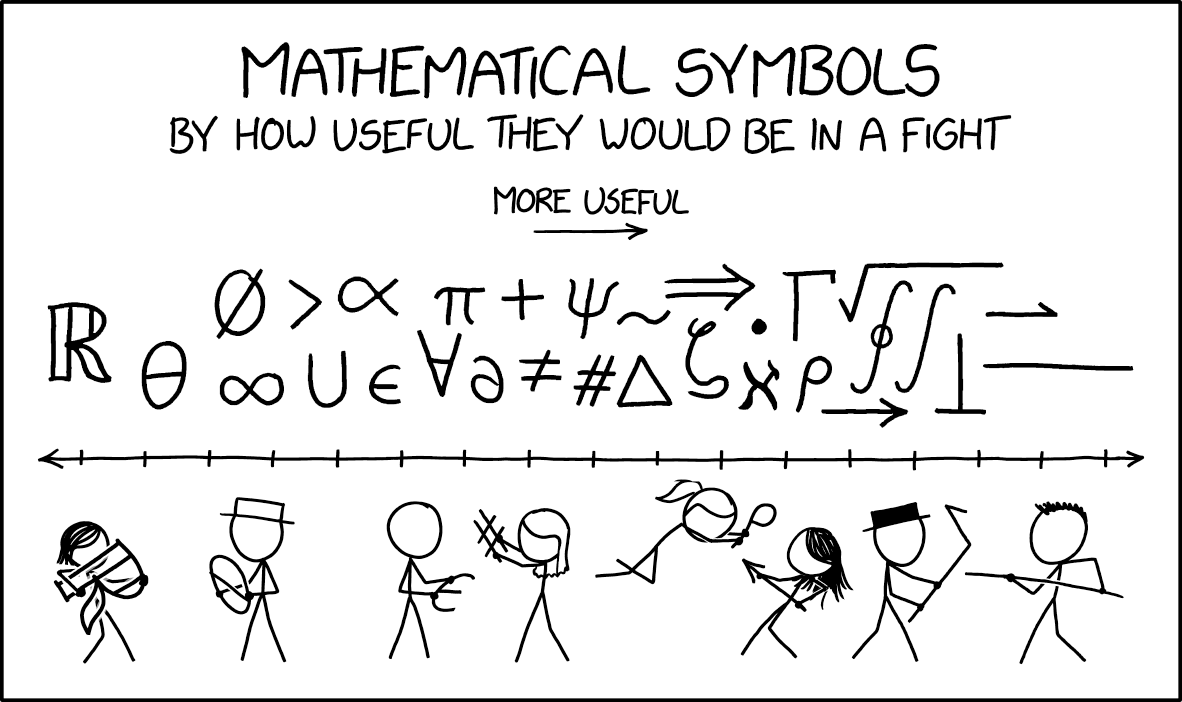
\includegraphics[width=\textwidth]{mathematical_symbol_fight_2x.png} % or tikz or anything
  \end{figure}
% xkcd_2343

As physicists the most important binary relation is none of those things\footnote{I thank Yuval Grossman teaching me this.}. What we usually care about is  $\sim$.\footnote{I use this the same way as $\propto$, which is completely different from `approximately,’ $\approx$.} The symbol $\sim$ tells us how how something \emph{scales}. If I double a quantity on the right-hand side, how does the quantity on the left-hand side scale? Does it depend linearly? Quadratically? Non-linearly? The answer encodes something important about the underlying physics of the system. The symbol $\sim$ the reason why \emph{imagine the cow is a sphere} is a popular punchline in a joke about physicists. 


Implicit in this discussion is the pragmatic policy that we will not care about stray factors of 2 in this class. As my adviser used to say, if you are worried about a factor of 2, then you have addition homework to figure out that factor of 2.\footnote{That being said, you are reading these notes and find an error, do let me know about it.} 

\section{Units}

There is another way in which physics is different from mathematics. It is far more prosaic. \emph{Quantities in physics have units}. We do deal in simply numbers, we deal with kilograms, electron volts, meters. It turns out that dimensional analysis is a big part of what we do as physicists. 

\begin{exercise}
Explain, in words, why the quantity $\sin(3~\text{cm})$ is absolute nonsense in any context. What about $\text{exp}(2~\text{kg})$?
\end{exercise}

\chapter{Dimensional Analysis}

You may be be surprised how far one can go in physics by thinking deeply about dimensional analysis. Here we only get started. To take the next step, you may read more about the Buckingham Pi theorem or applications in physics. I recommend any of the following:
\begin{itemize}
  \item \fullcite{doi:10.1119/1.1987069}
  \item \fullcite{doi:10.1119/1.4902882}
  \item \fullcite{doi:10.1119/1.3535586}
  \item \fullcite{Stevenson:1980ga}.
\end{itemize}
\textbf{Dimensional analysis}\index{dimensional analysis} is simply the idea that by keeping track of the units of physical quantities, we can learn quite a bit about how those quantities must show up in our physical laws.


\section{Converting Units}

Imagine that you have three apples. This is a number (three) an a unit (apple). The meaning of the unit depends on what you're using it to measure. For example, if apples are \$1 each, then you could use an apple as a unit of currency. The way to do this is to simply \emph{multiply by one}:
\begin{align}
  (3\text{ apples}) \times \left(\frac{\text{\$ 1}}{\text{apple}}\right)
  &= \$ 3 \ .
\end{align}
We have used the fact that the exchange rate is simply the statement that
\begin{align}
  1\text{ apple} &= \$1
  & \Rightarrow &&
  1 &= \frac{\$ 1}{1\text{ apple}} \ .
\end{align}
You can do a similar thing for [kilo-]calories or any other conversion rate. 

All that matters is that the conversion factor is a constant. The constants of nature make very good `exchange rates.' For example, high-energy physicists use \textbf{natural units}\index{natural units}:
\begin{align}
  \hbar = c = 1 \ .
\end{align}
At face value, this does not make sense. $\hbar$ has units of action, $c$ is a speed, and 1 is dimensionless. However, because nature gives us a \emph{fundamental} unit of action and a \emph{fundamental} unit of speed, we may use them as conversion factors (exchange rates),
\begin{align}
  c = 3 \times 10^{10}~\text{cm}/\text{s} \ .
\end{align}
If $c=1$, then 
\begin{align}
  1~\text{s} &=  3 \times 10^{10}~\text{cm} \ .
\end{align}
This connects a unit of time to a unit of distance. By measuring time, the constant $c$ automatically gives an associated distance. The physical relevance of the distance is tied to the nature of the fundamental constant: one second (or `light-second') is the distance that a photon travels in one second. Observe that this only works because $c$ is a constant. 

\section{Quantifying units}

We use the notation that a physical quantity $Q$ has \textbf{dimension}\index{dimension} $[Q]$ that can be expressed in terms of units of length, mass, and time:
\begin{align}
  [Q] = L^a M^b T^c \ .
\end{align}
The {dimension} is the statement of the powers $a$, $b$, and $c$. You may want to also include units of, say, electric charge. Sticklers may pontificate about whether electric charge formally carries a new unit or not. 


\begin{example}
What are the units of force? We remember that $\vec{F} = m\vec{a}$, so 
\begin{align}
  [\vec F] &= [m][\vec{a}] = M\times L T^{-2} = L^1 M^1 T^{-2} \ .
  \label{eq:02:force:units}
\end{align}
\end{example}

\begin{exercise}
What are the units of the fine structure constant?
\end{exercise}


When working in \textbf{natural units}, $c=1$ means that units of length and time are the same and $\hbar = 1$ means that units of time and energy (mass) are inversely related. In natural units, one simply writes $[Q]$ to mean the mass-dimension of a quantity. To revert back to conventional units, one simply multiplies by appropriate factors of $1=c$ and $1=\hbar$. 

\begin{example}
What are the units of force in natural units? From \eqref{eq:02:force:units} we multiply by one to convert length and time into mass dimensions:
\begin{align}
  [\vec F] &= [c^{-3} \hbar \vec{F}] = M^2 \ .
\end{align}
In natural units we say $[\vec F] = 2$. Recall that energy and mass have the same dimension, which you may recall from the Einstein relation $E^2 = m^2c^4 + p^2c^2$.
\end{example}

\section{Dimensional analysis at work}


\subsection{Sanity Check}

The simplest use of dimensional analysis is to check your work. The following expression is obviously wrong:
\begin{align}
  1 + (3~\text{cm}) \ .
\end{align}
This does not make sense. You cannot sum terms with different dimensions. Similarly, $\sin(3\text{ cm})$ does not make sense. What about $e^{5~\text{cm}}$? This doesn't make sense because
\begin{align}
  e^x = 1 + x + \frac{1}{2!} x^2 +  \cdots
\end{align}
Since each term comes with a different power of $x$, the argument of the exponential must be dimensionless. 

\begin{exercise}
Consider the energy spectrum of light emitted from some constant source---a distant star, the ongoing annihilation of dark matter in the galactic center, or a high-intensity laser. The spectrum encodes how many photons are emitted per unit time. We can plot this spectrum as a curve on a graph. We can even normalize the curve so that it integrates to one photon. This means we only care about the distribution of energy, not the absolute amount. The horizontal axis of such a plot is the photon energy. What are the units of the vertical axis?
\end{exercise}


\subsection{Solving problems}

Here is a common problem in introductory physics. Assume you have a pendulum with some sufficiently small initial displacement $\theta_0$. What’s the period, $\tau$ of the pendulum? We draw a picture like Fig~\ref{fig:simple_pendulum}.
%
\marginfig{figures/lec01_pendulum.pdf}{Sketch of a simple pendulum.}{fig:simple_pendulum}
%
%
From dimensional analysis, we know that the period has dimensions of time, $[\tau] = T$. The problem gives us a length $[\ell]=L$ and the gravitational acceleration, $[g]=LT^{-2}$. Note that $[\theta_0] = 1$ is dimensionless. This means that the only way to form a quantity with dimensions of time is to use $g^{-1/2}$. This leaves us with a leftover $L^{-1/2}$, which we can fix by inserting a square root of $\ell$:
\begin{align}
  \tau \sim g^{-1/2} \ell^{1/2} \ .
\end{align}
If we want to be fancy, we can make this an equal sign by writing a function of the other dimensionless quantities in the problem:
\begin{align}
  \tau = f(\theta_0) \sqrt{\frac{\ell}{g}} \ .
\end{align}

\flip{To do: include problems from Robinett AJP article on dimensional analysis, doi: 10.1119/1.4902882.}


\subsection{Scaling}

A key theme in physics is scaling relations. We present a somewhat contrived example of how this works adapted from section 11 of V.\ I.\ Arnold's \emph{Mathematical Methods of Classical Mechanics}.\footnote{This is one of my favorite differential geometry textbooks because it is disguised as a book on mechanics.}. Suppose you have some static, central potential $U(\vec r)$. Maybe it’s some planet orbiting a star. 
%
\textfig[1]{figures/lec01_orbit.pdf}{A orbital trajectory, $\vec{r}_0(t)$.}{fig:simple_orbit}
%
The force law gives:
\begin{align}
  m 
  \ddot{\vec{r}} = - \frac{\partial U}{\partial\vec{r}} \ .
  \label{eq:scaling:eg}
\end{align}
Suppose we are given a solution, $\vec r_0(t)$. Perhaps this is a trajectory that is experimentally verified. Dimensional analysis gives us a way to scale this solution into other solutions. For example, let us scale time by defining a new variable $t'$:
\begin{align}
  t \equiv \alpha t' \ .
\end{align}
Because the potential is static, then only the left-hand side of the force law changes. Even though the right-hand side formally has dimensions of time, $T^{-2}$, it does not transform because those units are carried in a constant, perhaps $G_N$, not a $(d/dt)^2$ like the left-hand side. The left-hand side of the force law gives:
\begin{align}
  m\left(\frac{d}{dt}\right)^2 \vec r_0(t) 
  &=
  m\alpha^{-2} \left(\frac{d}{dt'}\right)^2 \vec r_0(\alpha t') \ .
\end{align}
This begs us to define a new mass $m' = m\alpha^{-2}$ so that
\begin{align}
   m' \left(\frac{d}{dt'}\right)^2 {\vec{r}_0}(\alpha t')
  = - \frac{\partial U}{\partial\vec{r}_0} \ .
\end{align}
What this tells us is that we may define a new trajectory, $\vec r_1(t') \equiv \vec{r}_0(\alpha t')$, which is a solution in the same potential that traces the same trajectory but at $\alpha$ times the speed and with mass $m'$. Changing labels $t'\to t$ for a direct comparison:
\begin{align}
   m' \left(\frac{d}{dt}\right)^2 {\vec{r}_1}(t)
  = - \frac{\partial U}{\partial\vec{r}_1} \ ,
\end{align}
which is indeed\footnote{We were able to swap $\vec r_0$ with $\vec r_1$ simply because $U$ only depends on the position.} \eqref{eq:scaling:eg} with a new mass $m'$ and a trajectory $\vec r_1(t') \equiv \vec{r}_0(\alpha t')$. For example, if $\alpha = 2$, then $\vec r_1(t)$ traces the same trajectory at double the velocity with one fourth of the mass.

\begin{exercise} 
I missed something in the example above. In order for a planet of mass $m'$ to have trajectory $\vec r_1(t')$, what is the mass of the star compared to the original mass $M_\star$?\footnote{Thanks to Eric Zhang (2021) for pointing this out.} 
\end{exercise}

\begin{example} 
Business-y people like to quantify effort using words like `person--hour' or `person--years.' This is the idea that a 10 person--hour task would take 10 people one hour to complete, or one person 10 hours to complete, or 5 people two hours to complete, etc.  As you can see, this choice of units implies that effort has a linear scaling in both the number of people and the amount of time needed. Anyone who has worked on a group project knows that this linear scaling is bullshit. Frederick Brooks reflects on this in the 1974 essay, ``Myth of the Man--Month.''\sidecite{Brooks1975}
\end{example}

\subsection{Error Estimates}

This section is based on a lovely \emph{American Journal of Physics} article by Craig Bohren.\sidecite{doi:10.1119/1.1574042}%\footnote{\url{https://doi.org/10.1119/1.1574042}} 
Let us go back to another high school physics problem: we drop a ball of mass $m$ from height $h$. See Fig.~\ref{fig:simple_drop}. The task is to find the time $t_0$ for the ball to hit the ground.
%
\marginfig{figures/lec01_drop.pdf}{Dropping a ball of mass $m$.}{fig:simple_drop}

% Suppose you drop a mass $m$ from height $h$ that is initially at rest. How long before this hits the ground? 
You can integrate the force equation to get
\begin{align}
  t_0 = \sqrt{\frac{2h}{g}} \ .
\end{align}
This is the \emph{exact} answer \emph{within our model} of the system. The model made several assumptions: the mass is a point mass, the gravitational acceleration is constant at all positions, there is no air resistance, etc. In fact, we \emph{know} that if we do an experiment, our result will almost certainly \emph{not} be $t_0$. All we know is that $t_0$ is probably a good approximation of the actual answer. What we would like to to know is: \emph{how good of an approximation is it?}

One way to check this is to do the next-to-leading order (\acro{NLO}) calculation, taking into account a more realistic model and then compare to $t_0$. Of course, ``more realistic'' is also code for ``more complicated.'' Take a moment to appreciate that doing this is \emph{stupid}. Why do we need to do a \emph{hard} calculation to justify doing an \emph{easy} one? If we are going to do the hard calculation anyway, what was the point of ever doing the easy one?

What we really want is an error \emph{estimate}. The error\index{error} is
\begin{align}
  \epsilon &= \frac{t_1 - t_0}{t_0} \ .
\end{align}
This is a dimensionless quantity that determines how far off $t_0$ is from a more realistic calculation, $t_1$. Ideally we should not actually have to do much work to estimate $t_1$. 

Let us assume that we are not completely nuts and that we are in a regime where the error is small\footnote{Note the error has to be dimensionless in order for us to be able to call it `small,` otherwise it begs the question of `small with respect to what?'}. Then the error is a function of some dimensionless parameters, $\xi$, in the system. We define these $\xi$ so that as $\xi \to 0$, $\epsilon(\xi) \to 0$. In other words, the approximation gets better as the $\xi$ are made smaller. By Taylor expansion:
\begin{align}
  \epsilon(\xi) = \epsilon(0) + \epsilon'(0) \xi + \mathcal O(\xi^2) \ .
\end{align}
By assumption, $\epsilon(0) = 0$ and $\mathcal O(\xi^2)$ is  small. We can then make a reasonable \emph{assumption} that the dimensionless value $\epsilon'(0)$  is $\mathcal O(1)$. This tells us that the error goes like $\epsilon(\xi) \sim \xi$.

By the way $\mathcal O(1)$ is read ``order one'' and is fancy notation for the order of magnitude. Numbers like 0.6, 2, and $\pi$ are all $\mathcal O(1)$. A number like $4\pi$, on the other hand, is $\mathcal O(10)$.  The assumption that a dimensionless number is $\mathcal O(1)$ is reasonable. When nature gives you a dimensionless parameter that is both (a) important and (b) very different from $\mathcal O(1)$, then there's a good chance that it's trying to tell you something about your model. Good examples of this are the cosmological constant, the strong \acro{CP} phase, and the electroweak hierarchy problem.\footnote{There are also `bad' examples. The ratio of the angular size of the moon to the angular size of the sun is unity to very good approximation. This is quite certainly a coincidence. Our universe appears to be in an epoch where the density of matter, radiation, and dark energy all happen to be in the same ballpark. Our cosmological models imply that this is purely a coincidence. It would be very curious if this were not the case. As an exercise, you can critically explore the use of the anthropic principle in physics.} 

Here is how it works in practice. One effect that we miss in our toy calculation of $t_0$ is that the earth is round with radius $R$. This means that assuming a constant $g$ is an approximation. We have two choices for a dimensionless parameter $\xi$:
\begin{align}
  \xi &= \frac{h}{R}
  &\text{or}&&
  \xi &= \frac{R}{h} \ .
\end{align}
There is an obvious choice: $\xi = h/R$, because we know that as $h$ is made smaller (drop the ball closer to the ground) or $R$ becomes bigger (larger radius of Earth) then the constant $g$ approximation gets better. We thus expect that the corrections from the position-dependence of $g$ go like $\mathcal O(h/R)$.
 
% Exercise: check by explicit calculation, 2017 lec 1
\begin{exercise}
Check by explicit calculation that the correction to the constant $g$ approximation is linear in $h/R$. Start by writing the force law for a point source of at distance $r=R+h$ from the center of the Earth. Taylor expand to find a second order differential equation that is difficult to solve:
\begin{align} 
  \ddot{h} = \frac{-g}{\left(1+\frac{h}{R}\right)^2} \ .
\end{align}
Taylor expand to reduce this to an equation of the form
\begin{align}
  \frac{d^2 q}{ds^2} = -1 + 2q \ ,
\end{align}
Here we define the natural dimensionless variables, $q = h/R$ and $s = \left(g/R\right)^{1/2} t$. If the choice of $s$ is not obvious, please do everything in terms of $t$ and then observe that one can conveniently absorb a factor of $g/R$ into dimensionless time variables.\footnote{You should find an equation of the form $\ddot q = -(g/R)(1-\cdots)$.} Plug the dimensionless differential equation into \emph{Mathematica} or your favorite symbolic solver to obtain 
\begin{align}
  q(s) = c_1 e^{\sqrt{2}s} + c_2 e^{-\sqrt{2} s} + \frac{1}{2} \ .
\end{align}
Argue that the initial condition $\left.\dot h(t)\right|_{t=2} = 0$ implies that the coefficients satisfy $c_1 = c_2$ so that you can combine the exponentials into a hyperbolic cosine. 
% If $q_0$ is the value of $q(s)$ at $t=0$, show that $c_1 = (q_0  - 1/2)/2$.
Show that one obtains:
\begin{align}
  \frac{2q(s) - 1}{2q(0) -1} = \cosh(\sqrt{2}s) \ .
\end{align}
Argue why you can Taylor expand the right-hand side about small argument; that is, explain why $s \ll 1$. (Hint: use $h\ll R$.) Perform the Taylor expansion of the hyperbolic cosine to find that the leading correction to the fall time is
\begin{align}
  s_1 = \frac{2q_0}{1-2q_0} \ .
\end{align}
The zeroth order approximation was $s_0 = (g/R)^{1/2} t_0 = \sqrt{2q_0}$. Calculate $(s_1 - s_0)/s_0$ to confirm that this is $\mathcal O(h/R)$. 
\end{exercise}

\subsection{Bonus: Allometry}

There is a fun topic called \textbf{allometry}.\index{allometry} This is basically dimensional analysis applied to biology. A typical example is to consider two people who have roughly the same shape but different characteristic lengths, $\ell$ and $L$, Fig.~\ref{fig:lec1_allometry}.
\marginfig{figures/lec01_allometry.pdf}{Two mathematically similar people.}{fig:lec1_allometry}

% \begin{center}
% 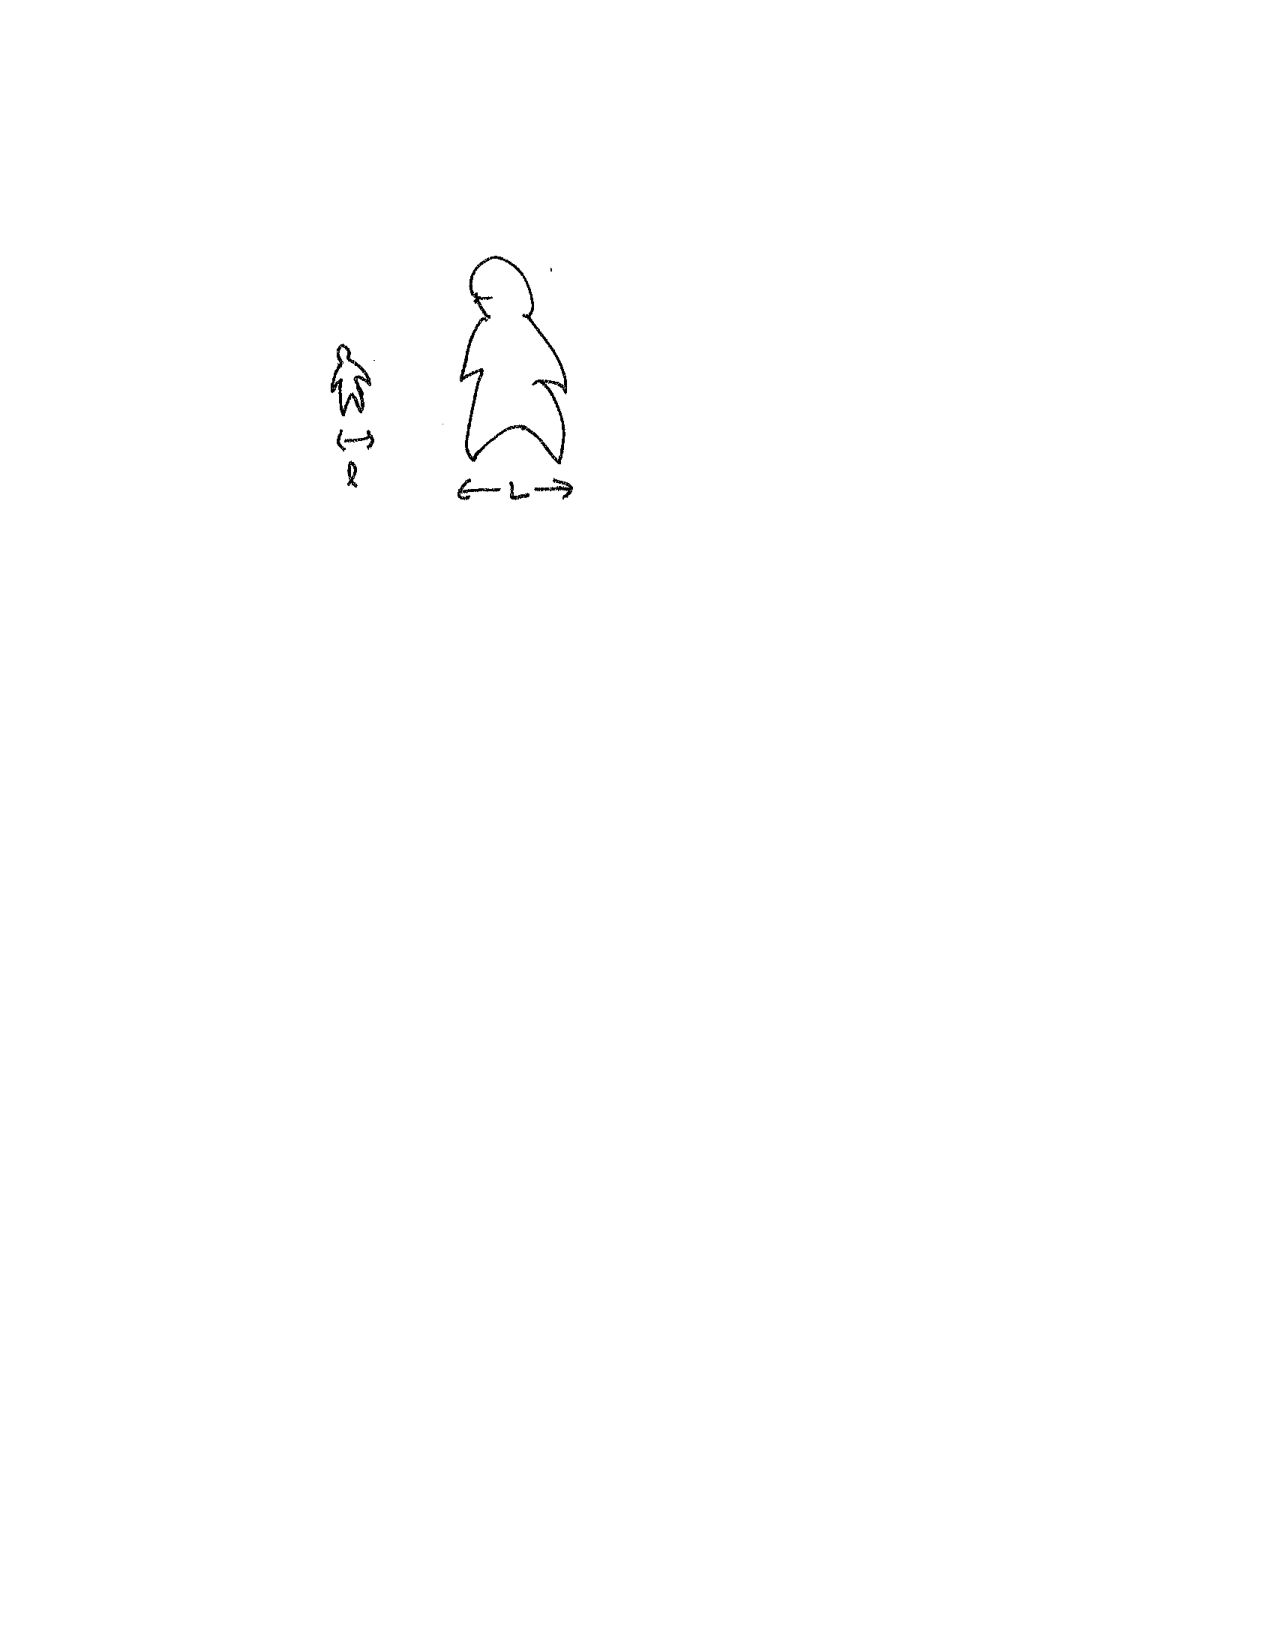
\includegraphics[width=.4\textwidth]{figures/lec01_allometry.pdf}
% \end{center}

\begin{exercise}
If both people exercised at the same rate, which one loses more absolute weight? By how much? Let us assume that weight loss is primarily from the conversion of organic molecules into carbon dioxide. 
\end{exercise}

\begin{exercise}
David Hu won his first IgNobel prize for determining that mammals take about 21 seconds to urinate, largely independently of their size\footnote{I learned about this in his excellent popular science book, \emph{How To Walk on Water and Climb Up Walls}.}. Can you use dimensional analysis to argue why this would be the case? It may be helpful to refer to the paper\sidecite{doi:10.1073/pnas.1402289111}. As you read it, figure out which terms are negligible (and in what limits), identify the assumptions of the mathematical model (scaling of the bladder and urethra), and prove the approximate scaling relation. Make a note to yourself of which steps were non-trivial and where one may have naively mis-modeled the system. By the way, David Hu won a second IgNobel prize for understanding wombats' cubical poop.
\end{exercise}

The above exercise on mammalian urination is a good example of \emph{modeling}.\index{model} As physicists, we must identify and make a mathematical model for the most salient features of a problem. We must also be able to quantify the error from neglecting sub-leading contributions. As a rough model for scaling purposes, we can ignore viscosity and surface tension effects on human-sized mammals. For much smaller mammals, these effects become larger---the authors of the study note that mice tend to urinate droplets---in which case one can ignore the `inertial' $\frac{1}{2} \rho v^2$ term in Bernoulli's equation. For human-sized mammals, we may assume that steady state urination is given by Bernoulli's equation:
\begin{align}
  P + \rho g h = \frac{1}{2}\rho v^2 \ ,
\end{align}
where $P$ is the pressure from the bladder, $h$ is the column height of the urethra, $\rho$ is the mass density of urine, and $v$ is the velocity of the urine at the end of the urethra. Let us simplify to the condition where urination is purely driven by gravity---that is, the bladder does not exert any additional pressure, $P=0$. You can now show that the total urination time scales like the mass of the mammal to the one-sixth power, $\tau \sim M^{1/6}$. That is, the urination time has a very weak scaling dependence on how massive the mammal is.

\begin{exercise}
In August 2021, Ezra Klein interviewed Dr.~C\'eline Goudner about the \acro{COVID-19} variant.~\sidecite{klein_2021} In the interview, Klein cited the statement that the Delta variant has $\mathcal O(1000)$ times the viral load than prior \acro{COVID} strains. Goudner then interprets this in the following way: if the \acro{CDC} defined `close contact' for prior strains as 15 minutes of being indoors with an infected invdividual without a mask, then the equivalent `close contact' time for the Delta variant is around \emph{one second}. What scaling assumptions go into that estimate? Some of these assumptions are not obvious to me: for example, parts of the respiratory have a fractal-like structure that would lead me to suspect fractal scaling dimensions for surface area. \acro{Remark}: Just because you know dimensional analysis, that does not make you a medical, healthcare, or public policy expert.\footnote{Early in the \acro{COVID-19} pandemic, many physicists became armchair  modelers of epidemics. Some of this was driven by hubris about our mathematical intuition. Many of the physicists lost interest when their models aligned poorly with what actually happened.} 
\end{exercise}

The following exercises draw from an article by Nicole Meyer-Verneta and Jean-Pierre Rospars in the American Journal of Physics\sidecite{doi:10.1119/1.4917310} and the references therein.
 \begin{exercise}
 Estimate the expected velocity of an All Terrain Armored Transport (\acro{AT}-\acro{AT})\footnote{\url{https://starwars.fandom.com/wiki/All_Terrain_Armored_Transport}} of characteristic height $L$. You can assume that the walking behavior is based on a pendulum. \acro{Answer}: $v \sim \sqrt{Lg}/2\pi$.
 \end{exercise}

 \begin{exercise}
 Based on the density $\rho$, the force-per-cross-sectional area $\sigma$, and the maximum rate of energy consumption per unit mass $b$, one may estimate the `sprint' velocity of an animal of length $L$. This sprint velocity is conveniently described with respect to the dimensionless `body lengths per time,' $v_\text{spr}/L$.

Remarkably, for over 20 orders of magnitude in animal length $L$, the value of $v_\text{spr}/L$ is within an order of magnitude of 10/sec:
% \begin{center}
%  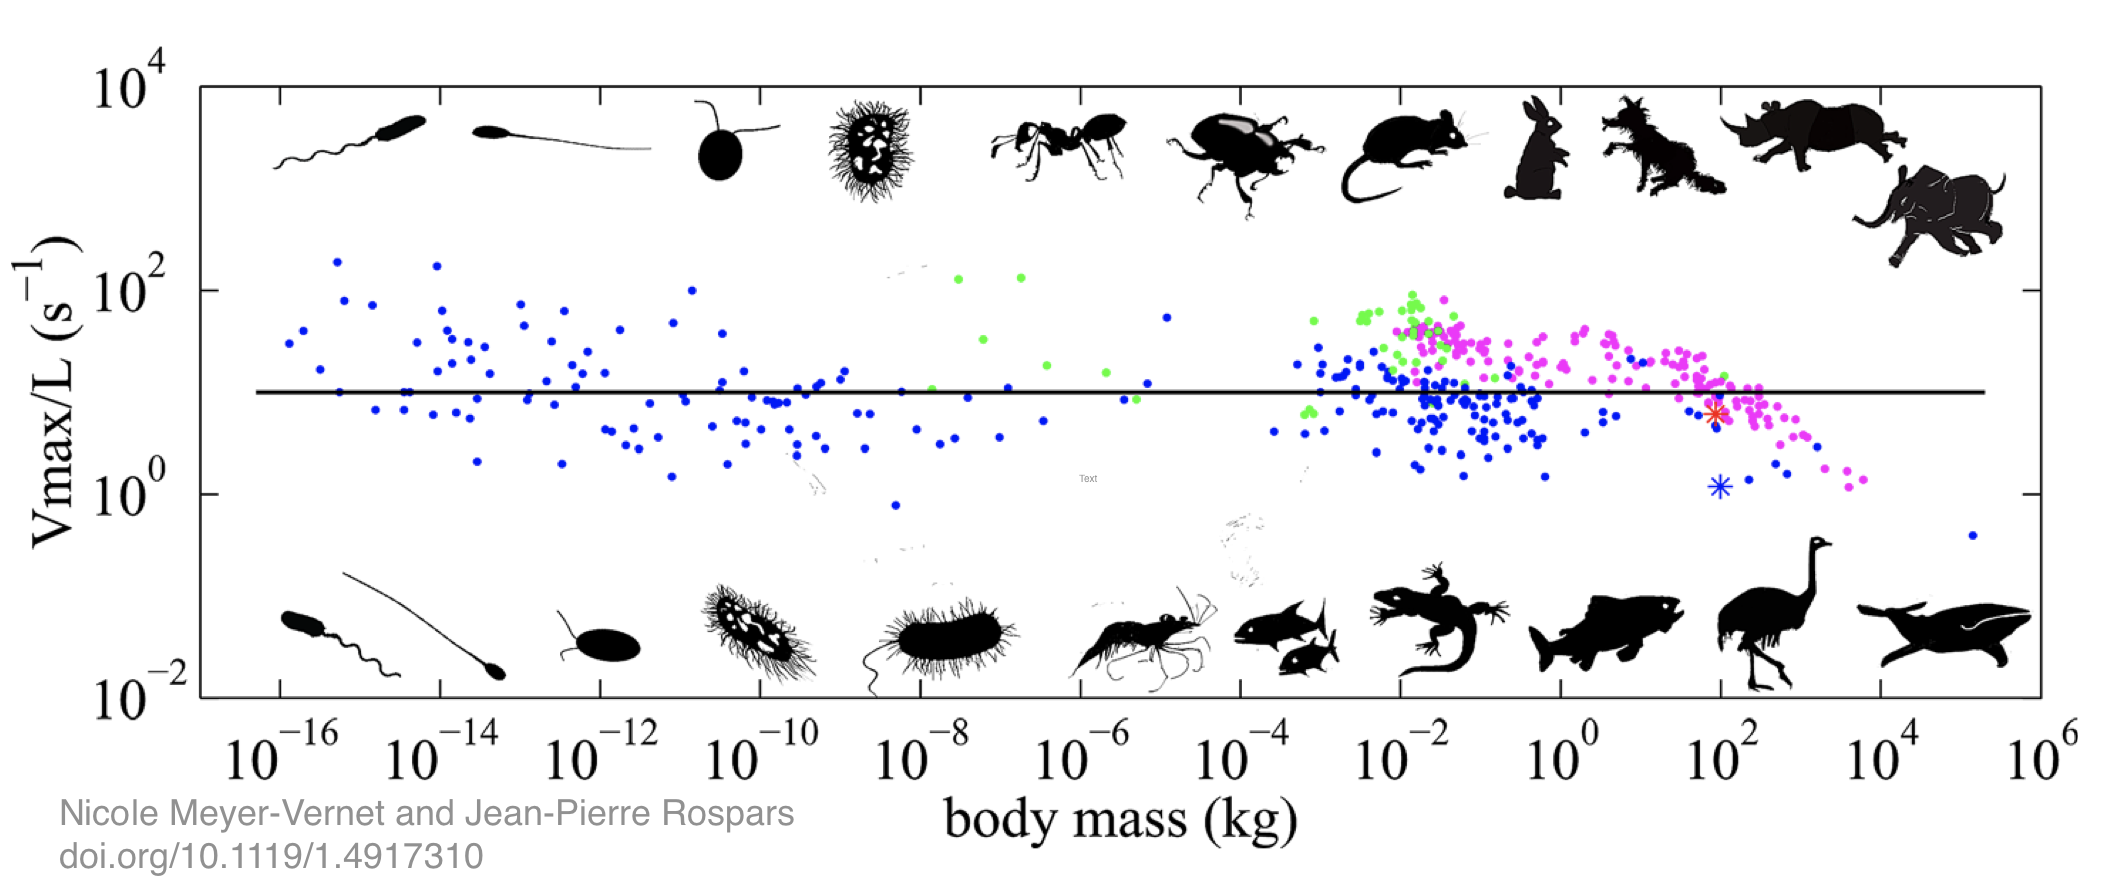
\includegraphics[width=.7\textwidth]{figures/allometry_meyer-verneta.png}
% \end{center}
\textfig[1]{figures/allometry_meyer-verneta.png}{Image from Meyer-Verneta and Rospars.~\cite{doi:10.1119/1.4917310}}{fig:allometry_meyer-verneta}


Argue from dimensional analysis that $v_\text{spr}/L \sim b\rho/\sigma$. (This is the easy part.) It turns out that there are simple physical principles for each of these terms to be roughly constant for all life on Earth (this is the more subtle part); see the article for a discussion.
\end{exercise}

\begin{exercise}
The height of trees. How does the maximum height of a tree, $L$ scale with the diameter of its cross section, $d$? For an argument that $L\sim d^{3/2}$, see Thomas McMahon's article ``The Mechanical Design of Trees'' in \emph{Scientific American} volume 233 (1975)\footnote{\url{https://www.jstor.org/stable/24949846}}. McMahon was the first to propose a physical explanation for the observed scaling law that the metabolic rate of an animal scales like the characteristic size to the 3/4 power. A nice bibliography of his work can be found in \emph{Annual Review of Biomedical Engineering}.~\sidecite{doi:10.1146/annurev.bioeng.3.1.0}
\end{exercise}


\part{Linear Algebra}

\chapter{Finite-Dimensional Linear Algebra}

\section{Yet another review of linear algebra}

Linear algebra is part of our physics \acro{DNA}. So why should we patronize ourselves with yet another review of linear algebra?
%
We want to understand Green’s functions as a matrix inverse. The `matrix' in question is the differential operator $\mathcal O$ in \eqref{eq:greens:function:equation}.
%
The identification boils down to the following:
\begin{align}
  \text{differential operator}
  &=
  \infty\text{-dimensional matrix} \ .
\end{align}
This is a poetic equal sign; for example, not every infinite dimensional matrix is a differential operator.\footnote{But by causality and locality these are the ones we care about in physics.} You may know matrices as a block of numbers that act on columns of numbers---\emph{vectors}---to produce another vector.
If differential operators are matrices, are vectors on which they act? These matrices act on a space of functions, which turns out to be a vector space:
\begin{align}
  \text{function space} &= \infty\text{-dimensional vector space} \ .
\end{align}
Again, the equal sign is poetic. 
Do not be intimidated by terminology like \emph{function space}; this is just an abstract place where functions live. Just recall back to your intuition from \acro{3D} Euclidean vector space, $\mathbb{R}^3$: any 3-vector $\vec{v}$ lives in the vector space $\mathbb{R}^3$. If we transform $\vec{v}$ by a linear transformation ${A}$, you get a new vector  $\vec{w} = {A}\vec{v} \in \mathbb{R}^3$ that is also in the vector space.

%
Weird things can happen when we extend our intuition from finite things to infinite things\footnote{For example, the Hilbert Hotel puzzle.}, but for this course we try to draw as much intuition as we can from finite dimensional linear algebra to apply it to infinite dimensional function spaces.



\section{What is Linear?}

A function\index{function}, $f(x)$, takes some kind of input $x$ and produces some kind of output. When the inputs and outputs are real numbers, $x,f(x)\in \mathbbm{R}$, then we can plot this relation between inputs and outputs on the $\mathbbm{R}^2$ by the mapping $(x,f(x))$. The curve $f(x)$ is the set of all points $(x,y) \in \mathbbm{R}^2$ such that $y=f(x)$. Said in yet another way, $y=f(x)$ is a constraint on $\mathbbm{R}^2$ that slices it into a one-dimensional subspace. To emphasize that $f$ takes in real numbers and spits out real numbers, we can write $f: \mathbbm{R}\to\mathbbm{R}$.

Before we end up getting too pedantic about what a curve is, recall that even children can tell you that the equation $f(x) = mx+b$ defines a line in the two dimensional plane. In this relation, $m$ is the slope and $b$ is the intercept of the line with the $y$-axis. We must be more restrictive: we set $b=0$ and impose that a linear relation between two numbers $x$ and $f(x)$ takes the form $f(x)=mx$. 

The reason for our apparent pedantry is to generalize the definition of {linearity} to extend beyond the picture of curves on $\mathbbm{R}^2$. A relation $f(x)$ is linear if the following are true:
\begin{align}
  f(\alpha x) &= \alpha f(x)\\
  f(x+y) &= f(x) + f(y) \ .
\end{align}
We assume that $x$ and $y$ are two objects of the same type, and $\alpha$ is simply some number.
\begin{exercise}
Confirm that $f(x)=mx$ is a linear function between real numbers for any value of $m\in \mathbbm{R}$.
\end{exercise}
We can state this all more formally. Suppose there is some collection of objects that we call $V$. Let $x$ and $y$ be two such objects: $x,y\in V$. Further, let $\alpha$ and $\beta$ be two numbers: $\alpha,\beta\in\mathbbm{R}$. Then a function $f:V\to W$ is \textbf{linear}\index{linear} if and only if\footnote{One can also write ``$\Leftrightarrow$'' to mean `if and only if.'}
\begin{align}
  f(\alpha x + \beta y) = \alpha f(x)+\beta f(y)
  \label{eq:def:linear}
\end{align}
Let us dissect this a bit. We stated that $x$ and $y$ have to be the same type of object, members of the class $V$. This echoes our discussion of dimensional analysis: if $x$ are apples and $y$ are Pokemon, then $2.5x+7y$ is nonsensical and so any function of such an object is nonsensical. We defined $\alpha$ and $\beta$ to be numbers\footnote{More generally, these are elements of a \textbf{field}: sets of objects with addition and multiplication defined.}: these just count how many objects in $V$ are being fed into our function. For now we assume that these are real numbers, but we will soon generalize to complex numbers. 

We wrote $f:V\to W$, which means that the output of the function $f(x)$ is an object of class $W$. In our toy example $f(x)=mx$, $V=W=\mathbbm{R}$. In general, $W$ and $V$ could be two totally different classes of objects. $W$ could be real numbers, something with units, a mathematical object with more structure, or any other class of objects. No matter what $V$ and $W$ are, the relation \eqref{eq:def:linear} tells us when a function is linear. 

\begin{example}
Let $f$ be a function that maps angles $\theta$ to rotation matrices,
\begin{align}
  R(\theta) = 
  \begin{pmatrix}
    \phantom{+}\cos\theta & \phantom{+}\sin\theta \\
    -\sin\theta & \phantom{+}\cos\theta
  \end{pmatrix} \ .
\end{align}
This map is not linear because
\begin{align}
  R(\theta_1 + \theta_2) \neq R(\theta_1) + R(\theta_2) \ ,
\end{align}
as you can check for the trivial case of $\theta_1 = \theta_2 = 0$.
\end{example}
\begin{exercise}
Let $f$ be a function that maps driving speed to the probability of being pulled over by the police or highway patrol. Explain why $f$ cannot be linear.
\end{exercise}

We can diagnose the linearity of a function, even when that function inputs and outputs objects that are more general than simply numbers. Thus far, we have been rather coy what it means to be an ``object in class $V$.'' This leads us to the notion of a vector space. 

\section{Vectors and Vector Spaces}

For our purposes in this course, we consider functions of \textbf{vectors}. Not all objects of interest are vectors, for example, coordinates are decidedly not vectors. The term \emph{position vector} is thus a faux pas.\footnote{Mathematicians chuckle at freshman physics textbooks.} On the contrary, infinitesimal differences of coordinates are vectors called \textbf{tangent vectors}. So what are vectors and vector spaces?

We focus on an imprecise, but physically intuitive working definition. For those who prefer a more mathematical discussion that is still tied to physical intuition, see \emph{Geometry, Topology, and Physics} by Nakahara.\sidecite{Nakahara:206619} A \textbf{vector}\index{vector} is an element of a vector space. That is, a \textbf{vector space}\index{vector space} is the `complete' collection of a given type of vector. 

We have already assumed that you can add vectors and rescale them by numbers; that is, we can take \textbf{linear combinations}\index{linear combination} of vectors. The assumption is implicit in our definition of linearity, \eqref{eq:def:linear}. Let $\vec{v}$ and $\vec{w}$ be any two vectors in the vector space $V$; we write this as $\vec{v},\vec{w}\in V$. Further, let $\alpha, \beta$ be numbers. We have the following rules:
\begin{itemize}
  \item The sum $\alpha\vec v + \beta\vec w$ is a vector in $V$. 
  \item The zero vector $\vec 0$ is a vector in $V$ such that $\vec 0 + \vec v = \vec v$. 
\end{itemize}
Formally there are other rules, but you probably already assumed them.\footnote{Please refer to your favorite linear algebra book.} These include the fact that vector addition is commutative, $\vec v + \vec w = \vec w + \vec v$, and associative, $(\vec v + \vec w) + \vec u = \vec v + (\vec w + \vec u)$. 
\begin{example}
The existence of a meaningful zero vector is one example why `position space' or coordinate space is not a vector space. The zero vector $\vec 0$ is the one that leaves other vectors unchanged upon addition: $\vec 0 + \vec x = \vec x$. Clearly this depends on the coordinate system and violates our intuition that physics should be independent of the choice of coordinates. Further, the notion of `adding positions' is physically nonsensical. On the contrary, differences of positions $\Delta{x} = \vec{x}_1-\vec{x}_2$ \emph{are} meaningful. For example, the force between two non-relativistic point particles depends the vector that is the difference between the particle positions.
\end{example}

\begin{exercise} \textbf{Color Space}. Colors for digital media have many representations. One popular representation is \acro{RGB} where the intensity of red, green, and blue components are specified. For example, $(25,174,40)$ is a pleasant shade of green. This triplet of numbers certainly looks like a vector: it is an ordered collection of numbers. Is the space of \acro{RGB} colors a vector space? \emph{Answer: no. Make a list of reasons why.} Like all meaningful questions, this rabbit hole runs deep; for example, see articles on the geometry of colors~\sidecite{weinberg1976geometry} or the overlapping sciences of physics and neurological perception of color~\sidecite{Logvinenko:2022}.
\end{exercise}

\section{Notation for Vectors}
\label{sec:vector:notation}

Physicists use a few different notations for vectors depending on the context. In these notes we also use whichever notation is most convenient for the task and we are not ashamed to change notation as needed. Students should be nimble to be able to make use of different notations.\footnote{As a student I was once very because a textbook introduced the notation $\overleftrightarrow{\partial}$. Only much later would I come to appreciate the perspicacity of that symbol.} It is absolutely critical that even though we can refer to a mathematical object with different notation, the underlying idea is the same. This insight is the key to never getting lost in the forest of special functions (Bessel, Legendre, spherical harmonics, etc.) that appear in physics.

\subsection{Bold/over-arrow notation} Thus far we refer to vectors with a boldfaced and italicized symbol,\footnote{See \acro{ISO 80000-2:2019} from the International Organization for Standardization.} $\vec{v}$. For the author this is a comfortable and familiar notation from school. On the board in a classroom, we sometimes write the vector with an underline $\underline{v}$ since boldfaced can be difficult to write freehand. A related notation uses arrows, $\overrightarrow{v}$. %Tensor $\tensor{T}$. ISO 80000-2:2019

\subsection{Ket notation} Another popular notation in physics is the bra--ket notation. Vectors are kets, $\ket{v}$. We we review below, there are also `row vectors' that we call bras, $\bra{w}$. This is all a tongue-in-cheek joke because you can combine a bra and a ket to form a \emph{braket}, $\langle w \,|\, v\rangle$, which we identify as the inner product (dot product) of two vectors $\langle w, v\rangle = \vec{w}\cdot\vec{v}$. 

\subsection{Index notation} A common metaphorical extension\footnote{\url{https://en.wikipedia.org/wiki/Metaphorical_extension}} in physics is the notation $v^i$. Technically, $v^i$ refers to the $i^\text{th}$ component of the vector $\vec{v}$.\footnote{$i^\text{th}$ component with respect to what? See the following section on basis vectors.} However, since physicists often write their equations component-wise, we often slip into the shorthand of using $v^i$ to mean either a given component or the entire vector. The appropriate meaning is usually clear from context. 

\subsection{Unadorned notation} We identify functions as vectors in an infinite dimensional space. In this case, it is often sufficient to avoid any additional adornment, so we write a function as $f$. The analog of a component of a vector, $v^i$, is the function at a point, $f(x)$.


\section{Basis Vectors}



The number of vectors in a vector space is formally infinite. If $\vec v$ is a vector, then so is $2v$ and $3v$, not to mention $0.999\vec{v}$, ad nauseum. Fortunately we can pick a standard set of reference vectors and define any other vector with respect to those reference vectors. We call those reference vectors \textbf{basis vectors} $\hat{\vec{e}}_{(i)}$ and the entire set a \textbf{basis}\index{basis} for the vector space.\footnote{Please humor the unusual notation with a lower index in parenthesis. We explain this unusual choice in Section~\ref{sec:indices}.} We may express any vector $\vec v$ in the vector space as a linear combination of basis vectors:
\begin{align}
  \vec{v} = \sum_i v^i\hat{\vec{e}}_{(i)} \ .
\end{align}
\begin{example}
In two dimensional Euclidean space, $\mathbbm{R}^2$ we have a canonical basis
\begin{align}
 \hat{\vec{e}}_{(1)} \equiv 
  \begin{pmatrix}
    1\\0
  \end{pmatrix}
  &&
 \hat{\vec{e}}_{(2)} \equiv 
  \begin{pmatrix}
    0\\1
  \end{pmatrix} \ .
\end{align}
\emph{Canonical} is just a fancy way to say \emph{the obvious choice}. The first basis vector points in the $x$ direction, the cond points in the $y$ direction. We can thus represent a vector $\vec{v}$ as a linear combination,
\begin{align}
  \vec{v} = 
  \begin{pmatrix}
    v^1 \\ v^2
  \end{pmatrix}
  =
  v^1\hat{\vec{e}}_{(1)} + v^2\hat{\vec{e}}_{(2)} \ .
\end{align}
We could have defined a different basis, for example
\begin{align}
 \hat{\vec{e}}_{(1)}' \equiv 
  \frac{1}{\sqrt{2}}
  \begin{pmatrix}
    1\\1
  \end{pmatrix}
  &&
 \hat{\vec{e}}_{(2)}' \equiv 
  \frac{1}{\sqrt{2}}
  \begin{pmatrix}
    \phantom{+}1\\-1
  \end{pmatrix} \ .
\end{align}
In this primed basis the vector $\vec{v}$ would have different components,
\begin{align}
  \vec{v} = v'^1\hat{\vec{e}}_{(1)}' + v'^2\hat{\vec{e}}_{(2)}' \ ,
\end{align}
where clearly $v'^i \neq v^i$.
\end{example}
\begin{exercise}
Suppose $v^1 = 3$ and $v^2 = -4.5$ in the unprimed basis from the example above. Find the corresponding primed components $v'^1$ and $v'^2$. You do not have to do this in any fancy systematic way. \emph{Suggestion}: just draw the vectors on $\mathbbm{R}^2$. You do not often get to do this, especially with more abstract vectors. But when you can do something the simple way, you should do it that way and then think about how to generalize `the simple way.'
\end{exercise}

The number of basis vectors required to describe any vector is called the \textbf{dimension}\index{dimension} of the vector space. The dimension of $\mathbbm{R}^2$ is two. If you specify fewer basis vectors than the dimension of the vector space, then there are vectors that you cannot describe. If you specify more basis vectors than the dimension of the vector space, then there is not a unique way to specify the vector components.\footnote{\emph{Then shalt thou count to three, no more, no less. Three shall be the number thou shalt count, and the number of the counting shall be three. Four shalt thou not count, neither count thou two, excepting that thou then proceed to three. Five is right out.} (\emph{Monty Python \& The Holy Grail}, 1975)}
\begin{example}
In $\mathbbm{R}^2$, suppose we specified \emph{three} basis vectors,
\begin{align}
 \hat{\vec{e}}_{(1)} \equiv 
  \begin{pmatrix}
    1\\0
  \end{pmatrix}
  &&
 \hat{\vec{e}}_{(2)} \equiv 
  \begin{pmatrix}
    0\\1
  \end{pmatrix} 
  &&
 \hat{\vec{e}}_{(3)} \equiv 
  \frac{-1}{\sqrt{2}}
  \begin{pmatrix}
    1\\1
  \end{pmatrix}
  \ .
\end{align}
The vector $\vec{v} =\hat{\vec{e}}_{(1)} +\hat{\vec{e}}_{(2)}$ can equivalently be written as $\vec{v} = -\sqrt{2}\vec{e}_{(3)}$.
\end{example}
\begin{exercise}
In the example above, write $\vec{v}$ with respect to the three basis vectors in a way that has not yet been specified. Repeat this exercise until it is obvious that there are an infinite number of ways of writing $\vec{v}$ with respect to the three basis vectors. Contrast this to the case where we restrict to any pair of the basis vectors, in which case the components of $\vec{v}$ are unique.
\end{exercise}

\section{Nice basis vectors}
\label{sec:nice:basis}

You have likely been trained to \emph{assume} that a basis is \emph{nice}, following the notion of assumed \emph{niceness}\footnote{Section~\ref{sec:niceness}.} in physics. As we move towards abstract vector spaces, it is worth explicitly stating these assumptions so that we can make a note of where they may break and what other mathematical structure we need to define them. The two assumptions are linear independence and orthonormality.

\subsection{Linear independence}

Two vectors $\vec{v}$ and $\vec{w}$ are \textbf{linearly independent}\index{linear independence} if they are not proportional to each other: $\vec{v} \neq \alpha \vec{w}$ for any number $\alpha$. The basis vectors for any reasonable basis are linearly independent---any given basis vector $\vec{e}_{(i)}$ cannot be written as a linear combination of the other basis vectors:
\begin{align}
\hat{\vec{e}}_{(i)} \neq \sum_{i\neq j}\hat{\vec{e}}_{(j)} \ ,
\end{align}
where the sum is over all basis vectors $\vec{e}_{(j)}$ except the $i^\text{th}$ basis vector. It should be obvious\footnote{In the sense of Section~\ref{sec:obvious}.} that a proposed basis with a linearly dependent basis vector
\begin{enumerate}
  \item Does not uniquely define the components of some vectors $\vec{v}$ in the vector space.
  \item Either has more basis vectors than the dimension of the space, or there are vectors in the space that cannot be described by the basis.
\end{enumerate}
Thus every basis vector in any reasonable basis is linearly independent from the other basis vectors.

\subsection{Orthonormality}

Okay, this is actually two different conditions: orthogonal and normal. The basis vectors of a nice basis are \emph{orthogonal} to every other basis vector and \emph{normalized} to have unit length. \textbf{Orthogonal} means that the vectors are perpendicular\index{orthogonal}. 

\emph{Eh...} then what do we mean by \emph{perpendicular}? We certainly have some notion of two directions being perpendicular from everyday life: north is perpendicular to west because if we move five steps north we are stationary in the east--west direction. But how do we define this mathematically? In fact, while we are at it: how do we define `unit length' with respect to these vectors?\footnote{From a physics perspective: in what units?} 

\begin{example}
Orthogonality and linear independence are related but are not the same. Orthogonal vectors are linearly independent, but linear independence does not imply orthogonality. For example, consider the basis of $\mathbbm{R}^2$:
\begin{align}
 \hat{\vec{e}}_{(1)} \equiv 
  \begin{pmatrix}
    1\\0
  \end{pmatrix}
  &&
 \hat{\vec{e}}_{(2)} \equiv 
  \begin{pmatrix}
    1\\1
  \end{pmatrix} 
  \label{eq:nice:basis:eg:e1e2}
  \ .
\end{align}
These vectors are obviously linearly independent. Assuming the usual Euclidean inner product, the are also \emph{not} orthogonal. The observant student will notice that linear independence does not require one to define an inner product, whereas orthogonality is only defined with respect to some inner product.
\end{example}
\begin{exercise}
Let $\vec{v}$ be the vector that is pointing in the $\hat{\vec{x}}$ direction of $\mathbbm{R}^2$.  What are the components of $\vec{v}$ with respect to the basis in \eqref{eq:nice:basis:eg:e1e2}? Similarly, let $\vec{w}$ be the vector that is pointing in the $\hat{\vec{y}}$ direction of $\mathbbm{R}^2$. What are the components of $\vec{w}$ with respect to the basis in \eqref{eq:nice:basis:eg:e1e2}?
\end{exercise}
Unlike linear independence, orthonormality is not a strictly necessary condition for having a basis---though it is hard to imagine a scenario where one would \emph{not} use an orthonormal basis. However, the notions of orthogonality and normalization depend on \emph{additional} mathematical structure that we have to impose/assume/invent for our vector space. Formally, we say that we promote the vector space to a \textbf{metric space}\index{metric space}. The additional structure that we define is a machine that takes two vectors and tells us something about the `distance' between them. We call this machine the \textbf{metric}\index{metric}, \textbf{inner product}\index{inner product}, or \textbf{dot product}\index{dot product}; each phrase refers to the same thing. Once we have a metric, the Gram--Schmidt procedure assures us that we can construct an orthonormal basis from a linearly independent basis, see Exercise~\ref{ex:gram:schmidt}. 


\section{The metric, inner product, or dot product}

The \textbf{metric} (inner/dot product product) on a real vector space $V$ is a bilinear\footnote{This simply means linear in each argument.} map from $V\times V\to \mathbbm{R}$.\footnote{We also care about \emph{complex} vector spaces, in which case the metric is a map from $V\times V\to \mathbbm{C}$.} This means that it is a machine that takes two vectors and returns out a number. We use the metric to measure one vector with respect to another. We further impose that the metric is symmetric: it should not matter whether we measure $\vec{v}$ with respect to $\vec{w}$ or vice versa: their `overlap' should be the same. 
%
We use the angle bracket notation where $\langle \vec{v},\vec{w}\rangle$ is the inner product of two vectors $\vec{v}$ and $\vec{w}$.\footnote{This is deliberately suggestive of the ket notation for vectors, Sec.~\ref{sec:vector:notation}.}
%
Summarizing the above properties in equations:
\begin{align}
  \langle \alpha \vec{v}+\beta\vec{w}, \vec{u} \rangle &=
  \alpha \langle \vec{v},\vec{u}\rangle +
  \beta \langle \vec{w},\vec{u}\rangle 
  \\
  \langle \vec{v}, \alpha \vec{w} + \beta \vec{u} \rangle &=
  \alpha \langle \vec{v},\vec{w}\rangle +
  \beta \langle \vec{v},\vec{u}\rangle 
  \\
  \langle \vec{v},\vec{w}\rangle  &=
  \langle \vec{w},\vec{v}\rangle  \ .
\end{align}
The \textbf{norm}\index{norm} of a vector is simply its length with respect to the metric. We write the norm of a vector $\vec{v}$ as $|\vec{v}|$, or sometimes as $||\vec{v}||$ when we really want to be fancy. The norm is simply the square root of the inner product of the vector with itself:
\begin{align}
  |\vec{v}| = \sqrt{\langle \vec{v}, \vec{v}\rangle} \ .
\end{align}
Because we want lengths to make sense, we make a further requirement that any sensible metric is \emph{positive definite},\footnote{Mathematicians use the adjective \textbf{Riemannian}\index{Riemannian} to mean `positive definite' when applied to metrics. Physicists often assume that their metrics are Riemannian.}
\begin{align}
  \langle \vec{v},\vec{v}\rangle > 0 
\end{align}
for any vector $\vec{v}\in V$. 
%
Both the angle bracket notation $\langle \vec v, \vec w \rangle$ and the dot product notation $\vec v \cdot \vec w$ make it clear that the metric is an operation between two vectors. There is another notation that highlights the idea of the metric as a map/function on $V\times V$:
\begin{align}
  g(\vec v, \vec w) = \langle \vec v, \vec w \rangle \ . 
\end{align}
The convention of calling the metric $g$ is common in general relativity.\footnote{Some suggest that the $g$ stands for `gravity' \url{https://hsm.stackexchange.com/questions/3435/}, see also \url{https://www.reddit.com/r/math/comments/p2i6qu/why_is_a_riemannian_metric_tensor_denoted_by_g/}.} 
% gram matrix

\begin{example} The Euclidean metric in Cartesian coordinates is the usual dot product from childhood. In $\mathbbm{R}^2$, the dot product of two vectors is $\vec{v}\cdot \vec{w} = v^1w^1 + v^2w^2$. The generalization to $\mathbbm{R}^N$ is
\begin{align}
  \langle \vec v, \vec w \rangle = g(\vec v, \vec w) = \vec v\cdot \vec w
  = \sum_{i=1}^N v^i w^i \ ,
  \label{ex:euclidean:R2:metric}
\end{align}
where $v^i$ and $w^i$ are the $i^\text{th}$ Cartesian components of the vectors $\vec v$ and $\vec w$ respectively. There are a few different ways of writing this out. 

Let $\vec v^\text{T}$ be the transpose of $\vec{v}$. We do not want to dwell on what this means (see below), but suffice it to say that if $\vec{v}$ is what a child would call a column vector, then $\vec v^\text{T}$ is what the child would call a row vector. The child may then say that the length of $\vec{v}$ is simply $$|\vec v| = \sqrt{\vec v^\text{T} \vec v}\ .$$ Observe that there is no inner product in this expression: the `row vector' $\vec v^\text{T}$ naturally acts on the column vector $\vec v$ by matrix multiplication.\footnote{As we discuss below, the row vector is a linear function from $V\to \mathbbm{R}$.} This suggests that the inner/dot product is related to
\begin{align}
  \vec v\cdot \vec w = \vec v^\text{T} \vec w \ .
\end{align}
To be fully general, we write
\begin{align}
  \vec v \cdot \vec w &\equiv \vec v^\text{T} \tens{g} \vec{w}
  &
  \tens{g} &= 
  \begin{pmatrix}
    1 & 0 \\
    0 & 1
  \end{pmatrix} \ .
  \label{eq:eg:R2:dot:product:matrix}
\end{align}
Other metrics on $\mathbbm{R}^2$ may be defined the components of the matrix $\tens{g}$. 

Yet another definition of the metric is with respect to the differential line element. For the Euclidean metric in $\mathbbm{R}^2$,
\begin{align}
  ds^2 = dx^2 + dy^2 \ .
\end{align}
This generalizes to the form
\begin{align}
  ds^2 = \sum_{i,j=1}^2 g_{ij} dx^i dx^j \ ,
  \label{eq:ds2:gij}
\end{align}
where $g_{ij}$ are the components of $\tens{g}$. Here the differentials are linear functions that take in one of the vector arguments of the metric and spit out a number.\footnote{Terms like $dx^2 = dx\otimes dx$ where the first $dx$ is a linear function of the first argument, and the second $dx$ is a linear function of the second argument.} This notation is familiar if you have studied some general relativity, but is likely completely mysterious for those with no exposure to differential geometry. Do not worry if you fare not [yet] familiar with the notation: take it as an indication that there are elegant connections between calculus and linear algebra that are waiting for you to discover them.
\end{example}

The above exercise motivates writing the inner product in \emph{tensor} notation\footnote{We deliberately postpone defining what we mean by tensor.},
\begin{align}
  g(\vec v, \vec w) \equiv \sum_{i,j} g_{ij} v^i w^j \ .
  \label{eq:metric:in:tensor:notation}
\end{align}
For the case of $\mathbbm{R}^2$ in Cartesian coordinates, \eqref{eq:metric:in:tensor:notation} matches \eqref{ex:euclidean:R2:metric} when we take the components of $g_{ij}$ to be 
\begin{align}
 g_{ij} = \delta_{ij} 
  \equiv
  \begin{cases}
  1 & \text{if } i=j \\
  0 & \text{otherwise}
  \end{cases} \ ,
\end{align}
where we define a cousin\footnote{Formally the Kronecker $\delta$ should have one upper and one lower index, as we discuss below. Our abuse of notation, however, is mostly harmless. Yes, that was a Douglas Adams reference.} of the Kronecker $\delta$.  If you are not familiar with summing over indices, please check this explicitly: \eqref{eq:metric:in:tensor:notation} has a double sum over indices $i$ and $j$, whereas \eqref{ex:euclidean:R2:metric} only has a single sum. The $\delta_{ij}$ thus collapses one of the sums by forcing one of the indices to be exactly the same as the other index. The $g_{ij}$ in \eqref{eq:metric:in:tensor:notation} is precisely the same as the one that shows up in \eqref{eq:ds2:gij}.


\begin{exercise}
Given the restriction that a metric is a bilinear function of two vectors, explain why a general $\mathbbm{R}^2$ metric may be written in the form 
\eqref{eq:eg:R2:dot:product:matrix}. Why can any bilinear function of two vectors in $\mathbbm{R}^2$ be written with respect to the four components of $\tens{g}$? What are the restrictions on the components of $\tens{g}$ given that metric is symmetric and positive definite?
\end{exercise}

\begin{example}
The two-dimensional Minkowski space metric in the standard basis is
\begin{align}
  \langle\vec{v},\vec{w}\rangle = v^0w^0 - v^1w^1 \ ,
\end{align}
where we use the standard relativistic notation that the components of a vector are labelled as
\begin{align}
  \vec v = 
  \begin{pmatrix}
    v^0 \\ v^1
  \end{pmatrix} \ ,
\end{align}
with $v^0$ being the time-like component. The generalization to $(d+1)$-dimensional Minkowski space\footnote{This is called $\mathbbm{R}^{(1,d)}$ or $\mathbbm{R}^{(d,1)}$. Occasionally we invoke spaces with more than one time dimension. Some maximally symmetric spacetimes with negative curvature---think of a Pringles potato chip---are described as surfaces in $\mathbbm{R}^{(2,d)}$.} is simply
\begin{align}
  \langle \vec{v},\vec{w}\rangle = 
  v^0w^0 - \overrightarrow{\mathbf{v}}\cdot \overrightarrow{\mathbf{w}} \ ,
  \label{eq:Minkowski:metric}
\end{align}
where $\overrightarrow{\mathbf{v}}$ are the $d$-dimensional spatial components and $\overrightarrow{\mathbf{v}}\cdot \overrightarrow{\mathbf{w}}$ represents the ordinary Euclidean inner product on space.
\end{example}

\begin{exercise}\label{ex:gram:schmidt}The \textbf{Gram--Schmidt} procedure. Given the two vectors
\begin{align}
\vec v &=
\begin{pmatrix}
     2\\0
\end{pmatrix}   
&
\vec w &=
\begin{pmatrix}
     -1\\-1
\end{pmatrix} \ ,  
\end{align}
derive an orthonormal basis on $\mathbbm{R}^2$ using the canonical\footnote{This is a fancy word that we take to mean `the usual choice.' In this case we mean the Euclidean metric.}\index{canonical} metric. You should not need instructions for how to do this, even if you do not remember the Gram--Schmidt procedure: there are only two vectors and only a small number of operations you can do with them.
\end{exercise}

\begin{exercise} The \textbf{Gram--Schmidt} procedure, generalized.
Based on the previous exercise, give instructions for how to systematically derive an orthonormal basis from a set of $d$ linearly independent vectors in a $d$-dimensional metric space. Does it matter what order you process the original $d$ vectors in this procedure?
\end{exercise}


\begin{exercise}\label{ex:polar:coordinates} Write out the Euclidean metric for polar coordinates in $\mathbbm{R}^2$, $(r,\theta)$. These are related to ordinary Cartesian coordinates by:
\begin{align}
  (x,y) &= (r\cos\theta, r\sin\theta) \ .
\end{align}
The answer is \emph{not} $\langle \vec{v},\vec{w}\rangle = v_rw_r + v_\theta w_\theta$. You know the Euclidean metric in Cartesian coordinates and you know the change of basis, so this is straightforward. 
\end{exercise}


\section{Inner product as a projection}

\flip{insert figure}

The inner product has a natural geometric interpretation as the projection of one vector onto the other. By the symmetry of the metric, $\langle \vec v, \vec w \rangle = \langle \vec w, \vec v \rangle$, it does not matter which vector is being projected onto the other. This projection gives a definition of the angle, $\theta$, between two vectors:
\begin{align}
  \langle \vec v , \vec w \rangle \equiv |\vec v| |\vec w| \cos \theta \ .
\end{align}
Writing everything explicitly in terms of the inner product:
\begin{align}
  \cos \theta = \frac{\langle \vec v , \vec w \rangle}{\sqrt{\langle \vec v , \vec v \rangle\langle \vec w , \vec w \rangle}} \ .
  \label{eq:cos:theta:def:wrt:inner:product}
\end{align}
This definition of the angle obviously matches what we expect for vectors in $\mathbbm{R}^2$. In fact, with a little bit of thought, it obviously matches what we expect for vectors in $\mathbbm{R}^d$ with $d>1$: The two vectors live in a two-dimensional subspace of $\mathbbm{R}^d$ and so the angle reduces to the $\mathbbm{R}^2$ case. What is nice about this definition is that \eqref{eq:cos:theta:def:wrt:inner:product} generalizes to \emph{any} inner product.\footnote{One place this shows up is the classification of continuous symmetry groups. \textbf{Dynkin diagrams}\index{Dynkin diagrams} indicate the `angles' between different directions in the space of symmetry transformations.} 

Given an orthonormal basis $\left\{\hat{\vec{e}}_{(i)}\right\}$,\footnote{The notation $\{\cdots\}$ refers to a set of objects. In this case we mean the set of basis vectors: $\hat{\vec{e}}_{(1)}, \hat{\vec{e}}_{(2)}, \cdots$. }, the components of a vector $\vec v$ with respect to this basis are simply the inner products:
\begin{align}
  v^i = \langle \hat{\vec{e}}_{(i)}, \vec v \rangle \ .
\end{align}
\begin{exercise}
Explain what goes wrong when the basis is not orthonormal. Give an explicit example in $\mathbbm{R}^2$. Define a non-orthonomal basis and a vector $\vec v$ with components $v^i$ with respect to the basis. Then take the inner products with the basis vectors to show that $v^i \neq \langle \hat{\vec{e}}_{(i)}, \vec v \rangle$.
\end{exercise}

Returning to our notion of a `nice basis' in Sec.~\ref{sec:nice:basis}, the orthonormality of a set of vectors is only defined with respect to a metric. A basis is orthonormal if
\begin{align}
  \langle \hat{\vec{e}}_{(i)}, \hat{\vec{e}}_{(j)} \rangle
  = \delta_{ij} 
  % \equiv
  % \begin{cases}
  % 1 & \text{if } i=j \\
  % 0 & \text{otherwise}
  % \end{cases} 
  \ .
\end{align}
% Here we have defined a cousin\footnote{Formally the Kronecker $\delta$ should have one upper and one lower index, as we discuss below. Our abuse of notation, however, is mostly harmless. Yes, that was a Douglas Adams reference.} of the Kronecker $\delta$. 
Conversely, given an orthonormal set of basis vectors the components of the metric $g_{ij}$ are,\footnote{This is sometimes callsed the \textbf{Gram matrix}} 
\begin{align}
  g_{ij} = \langle \hat{\vec{e}}_{(i)}, \hat{\vec{e}}_{(j)} \rangle \ .
\end{align}
This identification is obvious upon invoking the linearity of the inner prodcut and the expansion of any vector as a linear combination of basis vectors:
\begin{align}
  \langle \vec v, \vec w \rangle = 
  \left\langle
    \sum_i v^i \hat{\vec{e}}_{(i)},
    \sum_j w^j \hat{\vec{e}}_{(j)},
  \right\rangle
  =
  \sum_{i,j}
  v^iw^j\left\langle
     \hat{\vec{e}}_{(i)},
    \hat{\vec{e}}_{(j)},
  \right\rangle
  = 
  \sum_{i,j}
  g_{ij}v^iw^j
   \ ,
\end{align}
where the last equality identifies the metric components $g_{ij}$ in \eqref{eq:metric:in:tensor:notation}. The metric, which gives us a sense of angle and length, encodes nothing more and nothing less than the inner products of the basis vectors.

\begin{exercise}
Show that a basis is linearly independent if and only if
\begin{align}
\det\,\langle \hat{\vec{e}}_{(i)}, \hat{\vec{e}}_{(j)} \rangle \neq 0 \ .  
\end{align}
\end{exercise}
Because the metric is symmetric, it turns out\footnote{This phrase is code for ``you can prove it, but we do not prove it here.''} that one can always choose a basis where the metric is diagonal. This is tantamount to saying that there is an orthogonal basis. One can further impose that $|\det g_{ij}| = 1$ for an orthonormal basis.\footnote{The absolute value is important here because the  spacetime metric has a relative sign between timelike and spacelike components,~\eqref{eq:Minkowski:metric}.}

You may suspect that all this implies that there is always a \emph{correct} basis---or a class of correct bases---where the metric is always nice and diagonal. For many cases this is true and this is the origin of funny prefactors that show up in some of the standard mathematical expressions we use. However, there are exceptions to this. In general relativity, the statement that one can always diagonalize the metric is a \emph{local} statement. Physically this is equivalent to saying that at every point in spacetime one can chose a local inertial frame that is `free falling.' That is to say that even in a curved spacetime, at a given point you can choose coordinates where everything is Minkowski. However, the coordinates in which everything is `flat' at point $p$ do not generally match the coordinates in which everything is `flat' at point $q\neq p$. The mismatch between these coordinate systems is at the root of the mathematical structure of general relativity: it is the physical origin of the notions of connection (covariant derivative), parallel transport, and moving frames.\footnote{An excellent introduction that is grounded in physical intuition is Carroll's \emph{Spacetime and Geometry}. The appendices are a crash course in a graduate differential geometry course.}



\section{Linear functions of vectors}

Recalling our definition of linearity in \eqref{eq:def:linear}, we now focus on the class of linear functions that take in a vector and spit out a number. To say that mathematically, we consider linear functions from $V\to \mathbbm{R}$. This class of functions turns out to be significant enough to have a name. In fact, it is so significant that it has several names---and we do not always make it clear that we mean the same thing: \textbf{row vector}\index{row vector}, \textbf{bra}\index{bra}, \textbf{covariant vector}\index{covariant vector}, \textbf{one-form}\index{one-form}, \textbf{dual vector}\index{dual vector}, \textbf{covector}\index{covector}.\footnote{In japanese the prefix \emph{ko}- means `little.' That has nothing to do with the `co' in `covector,' but I recently learned about \emph{ko} in the context of the San-X characters Rillakuma and Korillakuma. The characters are delightful, but do not confuse yourself by thinking that vectors and covectors are related in the same way that Rillakuma and Korillakuma are related. It is really not even clear to me how the latter two are related.} All of these refer to the same idea of being a linear function on vectors that returns a number. By the way, there is a corresponding plurality of names for what we have thus far been calling a vector: column vector, ket\index{ket}, and \textbf{contravariant vector}\index{contravariant vector} all mean `vector.' 

The prototypical example here is a row vector. If we write a vector as a column of $N$ numbers,
\begin{align}
   \vec v = 
   \begin{pmatrix}
     v^1 \\
     \vdots \\
     v^N
   \end{pmatrix} \ ,
 \end{align}
 then a row vector $\tilde{\vec w}$ is---no surprise here---a row of $N$ numbers:
\begin{align}
  \tilde{\vec w} = 
  \begin{pmatrix}
    w_1, w_2, \cdots, w_N
  \end{pmatrix}\ ,
\end{align}
where we have very deliberately written the components with a lower index. We recall that the elementary school rule for matrix multiplication between two objects $\tilde{\vec w}$ and $\vec v$:
\begin{enumerate}
  \item Rotate the first object by $90^\circ$ in the clockwise direction. This means that $\tilde{\vec w}$ is rotated into a column of numbers.
  \item Multiply the elements of the two objects that are the same height. In this case, we multiply $w_1$ by $v^1$, $w_2$ by $v^2$, and so forth. 
  \item Sum together these multiplications: $w_1v^1 + w_2v^2 + \cdots$.
\end{enumerate}
\flip{insert figure}
In this way, the row vector $\tilde{\vec w}$ acts on the column vector $\vec v$ as
\begin{align}
  \tilde{\vec w} \vec v = \sum_i w_iv^i \ ,
  \label{eq:dual:vec:act:on:vec}
\end{align}
for some numbers $w_i$. The right-hand side here is clearly a number. Furthermore, it should be clear that the right hand side depends linearly on both $\tilde{\vec w}$ \emph{and} on $\vec v$. This means if we replace $\tilde{\vec w}$ with $2 \tilde{\vec w}$, then the number on the right-hand side doubles, and similarly with $\vec v$. In fact, we can be even more explicit about the role of $\tilde{\vec w}$ as a function that takes in vectors by writing this action as $\tilde{\vec w}[\vec v]$.

\begin{exercise}
Show that the space linear functions that map $V\to \mathbbm{R}$ is also a vector space with the same dimension as $V$. We call this the \textbf{dual vector space}, $V^*$.\index{dual vector space} Two thoughts should occur to you:
\begin{enumerate}
  \item The word `dual' seems to imply that the linear functions on $V$  are somehow identical\footnote{Perhaps a more mathematical word is `isomorphic.'} to the vectors in $V$.
  \item The prior point is `obvious' from the elementary school perspective that row vectors are simply column vectors that have been written horizontally.
\end{enumerate}
\end{exercise}



\subsection{Basis row vectors}

We can define a basis of row vectors/one-forms/bras/covariant vectors analogously to the basis of vectors. In the boldface notation, we could write these as $\tilde{\vec{e}}^{(i)}$ so that a row vector $\tilde{\vec w}$ may be expanded as
\begin{align}
 \tilde{\vec w} = \sum_i w_i \tilde{\vec{e}}^{(i)} \ ,
\end{align}
where we observe the careful placement of indices. The $w_i$ are simply the components of the row vector with respect to the specified basis. These components are simply numbers. All of the \emph{row-vector-ness} of a row vector is carried in the basis row-vectors. Everything that makes a given row vector unique is specified in the components $w_i$ that specify a particular linear combination of basis row-vectors.

In principle one can choose any set of basis row vectors satisfying linear independence. Obviously we prefer to have an orthonormal basis\footnote{If you are paying close attention you notice that we have not yet defined an inner product for the row vectors. Such an inner product is necessary to define `orthonormality' on this space of row vectors.}

We underline the following point:
\begin{quote}
If you know the what the basis objects do, then you know everything about the space.
\end{quote}
Given an orthonormal basis $\left\{\hat{\vec{e}}_{(i)}\right\}$ for the vector space $V$, there is a natural choice for a nice basis for the dual vector space $V^*$ of row vectors/dual vectors/bras/covariant vectors/one-forms.\footnote{Is it clear that these are all the same things? We can then just call them dual vectors or bras.} These are the basis linear functions that satisfy:
\begin{align}
  \tilde{\vec e}^{(i)} \left[\hat{\vec{e}}_{(j)}\right] = \delta^i_j
  \equiv
  \begin{cases}
  1 &\text{if } i=j\\
  0 &\text{otherwise} \ .
  \end{cases}
  \label{eq:canonical:dual:basis}
\end{align}
We read this as a basis dual vector $\tilde{\vec e}^{(i)}$ acting\footnote{I always thought about this as Pac-Man eating the ghosts.} on a basis vector $\hat{\vec{e}}_{(j)}$.
This canonical choice of basis realizes the rule \eqref{eq:dual:vec:act:on:vec} with the coefficients $w_i$ identified as the components of $\tilde{\vec w}$.

$\delta^i_j$ is the Kronecker $\delta$\index{Kronecker delta} with one upper and one lower index. When summing over the Kronecker $\delta$ with respect to either index, it enforces that the term only contributes when the two indices match. It replaces the sum over $i$ with a fixed value $i=j$, and vice versa.


\subsection{Creating dual vectors with a metric}

Let us be very clear: these dual vectors (row vectors, one-forms, bras, covariant vectors) \emph{do not require a metric}. The metric takes in two vectors and spits out a number, $V\times V\to \mathbbm{R}$. A row vector takes in a single vector and spits out a number, $V\to\mathbbm{R}$.\footnote{This is a good place to remind ourselves that eventually we replace $\mathbbm{R}$ with the complex numbers, $\mathbbm{C}$. One may further generalize to different \emph{fields}---generalizations of `numbers'.} These are two very different classes of objects. 

However, if our vector space happens to be a metric space---that is, if we happen to have a metric lying around that we care to attach to $V$---then we can use the metric to create dual vectors out of vectors. 
\begin{exercise}
If you do not already know the answer, then pause and take a moment to think how you would create a linear function from $V\to \mathbbm{R}$ given a bilinear function from $V\times V\to \mathbbm{R}$. This is a good way to check if you are parsing this information actively or if you have fallen asleep.\footnote{\emph{Inception} (2010), Christopher Nolan.} 
\end{exercise}

The idea is that we can \emph{pre-load} the metric with a vector. Pick any vector, $\vec{v}$. Now insert $\vec v$ into the first argument of the inner product, $\langle \vec v , \texttt{\textvisiblespace}\rangle$. This object now takes in a vector to fill in the second argument of the inner product and uses the machinery of the inner product to spit out a number. By the linearity of the inner product, $\langle \vec v , \texttt{\textvisiblespace}\rangle$ is a linear function from $V\to \mathbbm{R}$. This is precisely a dual vector. In fact, let us give this object a name:
\begin{align}
  \tilde{\vec v} = \langle \vec v , \texttt{\textvisiblespace}\rangle \ .
  \label{eq:tilde:v:as:transpose:metric}
\end{align}
Ta-da! We have successfully constructed a dual vector out of a vector. What are the components of this dual vector? Assuming the canonical basis for the dual space \eqref{eq:canonical:dual:basis}\footnote{This is by construction: we only have the basis of $V$ and create a basis for $V^*$ out of it.}, we can find the components of a dual vector by feeding it basis vectors:
\begin{align}
  \tilde{\vec v}\left[\hat{\vec e}_{(i)}\right]
  = 
  \sum_j v_j \tilde{\vec e}^{(j)} \left[\hat{\vec e}_{(i)}\right]
  = 
  v_j \ .
\end{align}
Applying our definition of $\tilde{\vec v}$ as a pre-loaded metric \eqref{eq:tilde:v:as:transpose:metric},
\begin{align}
\tilde{\vec v}\left[\hat{\vec e}_{(i)}\right]
= 
\sum_j v^j \langle\hat{\vec e}_{(j)},\hat{\vec e}_{(i)}\rangle  
= v^i \ .
\end{align}
From this we find that $v_j = g_{ji} v^i$, where we have used the tensor notation of the metricm \eqref{eq:metric:in:tensor:notation}. For the Euclidean metric where $g_{ji} = \delta_{ji}$ we have $v_i = v^i$: that is, the row vector has the same components as the column vector from which it was created. We now recognize that this operation of `pre-loading a metric' with a vector to create a dual vector is simply what we had been calling the \textbf{transpose}\index{transpose} of a vector:
\begin{align}
  \vec v^\text{T} = \tilde{\vec v} = \langle \vec v , \texttt{\textvisiblespace}\rangle \ .
  \label{eq:transpose:as:inner:product:preloaded}
\end{align}
There is a generalization of the transpose to complex vector spaces called the \textbf{Hermitian conjugate}, which is the combined transpose and complex conjugation.\index{Hermitian conjugate} The symbol is the dagger, $\vec{v}^\dag = \tilde{\vec v}$. If you are not sure whether a space is real or complex, you can say Hermitian conjugate to cover both cases and sound fancy.\footnote{This reminds me of people who say \emph{compote} instead of \emph{jam}.}

We recognize that if the metric is not simply $g_{ij} = \delta_{ij}$, then the components of the dual vector are different from the components of the vector.\footnote{We know that we can diagonalize the metric with an auspicious choice of basis. However, there are plenty of non-trivial diagonal metrics. Consider Minkowski space or polar coordinates.} We can appreciate the utility of the upper and lower indices: something with an upper index is a component of a vector, while something with a lower index is a component of a dual vector. We can use the metric to convert from vectors to dual vectors, and the action on the components is clear: $v_i = \sum_i g_{ij}v^j$. In other words, the metric $g_{ij}$ is a machine that can lower indices.

Please appreciate that the phrase `lower the index' is really shorthand for \emph{convert the components of a vector into the components of the associated dual vector by taking the transpose/pre-loading the metric with that vector.} It is kind of a mouthful, so we say `lower the index' as a shortcut. Sometimes we even \emph{think} about the metric as acting on the indices of the components. But this too is a mental shortcut for understanding that we are moving between elements of a vector space and linear functions on those vectors.

\subsection{Bra and Ket notation}

The utility of the bra/ket notation in quantum mechanics is now evident. A vector is written as a ket, $\vec v = \ket{v}$. A dual vectors are written as a bra, $\tilde{\vec w} = \bra{w}$. The basis bras and kets are written as follows:
\begin{align}
  \ket{v} &= v^i\ket{i} &\Leftrightarrow&&
  \vec{v} &= v^i \hat{\vec e}_{(i)}
  \\
  \bra{w} &= w_j\bra{j} &\Leftrightarrow&&
  \tilde{\vec{w}} &= w_j \tilde{\vec e}^{(j)} \ .
\end{align}
One downside of the notation is that you have to mentally remember that the basis bra $\bra{j}$ is secretly a lower index while the basis ket $\ket{i}$ is secretly an upper index. On the other hand, the notation has the feature of connecting a vector to its transpose\footnote{We should really say `Hermitian conjugate' because the bra/ket notation is most commonly used for Hilbert spaces, which are complex vector spaces.}. Given a ket $\ket{v}$, there is a natural understanding what the corresponding bra is with respect to the inner product:
\begin{align}
  \bra{v} = \langle v | \texttt{\textvisiblespace} \rangle \ ,
\end{align}
where it is understood that the action of $\bra{v}$ on $\ket{w}$ is
\begin{align}
  \bra{v}\left[\ket{w}\right] = \langle v | w\rangle = \langle v, w \rangle \ .
\end{align}
We emphasize that $\langle v | w\rangle$ is a bra acting on a ket, wheras $\langle v | w\rangle$ is the inner product of two kets.


\subsection{The form notation}

A separate notation for vectors and dual vectors is inspired by differential geometry: 
\begin{align}
  \vec{v}=v^i \hat{\vec{e}}_{(i)} &\leftrightarrow v^i \frac{\partial}{\partial x}_i
  &
  \tilde{\vec w}=w_i \tilde{\vec{e}}^{(i)} &\leftrightarrow w_i dx^i \ .
\end{align}
The notation is perplexing the first time you see it. Everything looks familiar from calculus, but is now being used in a completely unusual context. Somehow:
\begin{itemize}
   \item Partial derivatives are the basis vectors. How odd! Partial derivatives are supposed to act on functions. Evidently the elements of the vector space are linear combinations of partial derivatives. 
   \item The infinitesimal elements, for example $dx$ or $dy$, are dual vectors. This is even more strange. Based on our intuition from freshman physics, there is no sense in which an ``infinitesimal displacement'' acts on a partial derivative to spit out a number! Though it is perhaps fair to say that the linear combination of infinitesimal displacements is still an infinitesimal displacement---whatever that means.
 \end{itemize} 
 \begin{exercise}
 Confirm that the set of partial derivatives $\partial_x$, $\partial_y$, $\partial_z$ form a three-dimensional vector space. Here $\partial_x = \partial/\partial x$ and so forth. The vector space is the space of first order partial derivative operators acting on a function. This is trivial: do linear combinations of these operators live in the space? If you are caught up on ``but what are these operators acting on?'' then you are focused on the wrong thing.
 \end{exercise}
 This all implies further structure that we have not specified. The further structure is the idea of a bundle over a manifold. We give a hint of this in Chap.~\ref{chap:vector:fields}.

 Let us be clear. We are \emph{defining} the object $dx$ as a basis for linear functions acting on the vector space of partial derivatives. In this context, we call these row vectors \textbf{differential one forms}\index{differential one forms}. The action of a differential one-form on a partial derivative is
 \begin{align}
   dx^i\left[\frac{\partial}{\partial x^j}\right] \equiv \delta^i_j \ ,
 \end{align}
 which you already know from \eqref{eq:canonical:dual:basis}. The utility of this notation is illuminated in the places where differential geometry intersects with physics. We present the notation here for those who anticipate meeting this formalism in the near future: by emphasizing that this curiosity is nothing more than vectors and dual vectors, they may then focus on the ways in which this story plays out on differential manifolds.\footnote{Manifold is another fancy word for what physicists usually call space or spacetime. It is like saying \emph{pommes frites} instead of \emph{french fries}.} 
 

\section{Summation convention}

From now on we invoke the summation convention that is standard in special and general relativity:
\begin{quote}
Whenever you see exactly one upper index that is the same as exactly one lower index, there is an implied sum over that index.
\end{quote}
This is the notational equivalent of tipping at a restaurant in the United States: you are never explicitly told to tip, but it is implied that a tip for the server should added to the final bill.\sidecite{segrave2009tipping}

The summing over two indices is called \textbf{contraction}\index{contraction} of these indices. This comes from the mental shorthand of replacing (dual) vectors with their components. If we think of $\vec{v}$ as $v^i$ and $\tilde{\vec{w}}$ as $w_i$, then we can think of the action of $\tilde{\vec w}$ on $\vec v$ as a contraction of the indices of their components:
\begin{align}
  \tilde{\vec w}\vec{v} = w_i v^i = w_1v^1 + w_2v^2 + \cdots \ ,
\end{align}
where we are using the summation convention on the right hand side.
%
The summation convention comes about from the observation that there are only certain ways in which objects in linear algebra can combine. It is incredibly useful and saves several pen/pencil/chalk/keystrokes,\footnote{Nevermind the indignities of using a whiteboard.}, but leads to the common mental shorthand that an object \emph{is} its components.\footnote{A vector $\vec{v}$ is fully specified by its components $v^i$ once you agree on a basis. However, the vector is not its components. The components tell you the specific linear combination of basis vectors.}

\begin{exercise}
Which of the following is an appropriate use of the summation convention? Anything that is not appropriate is nonsense and should ideally never appear in your work.
\begin{align}
  % v^i w^k g_{ik} &= v^1w^1g_{11}+v^2w^1g_{21} + \cdots + v^1w^2g_{12} + \cdots
  % \\
  v^i w^i &= w^1 v^1 + w^2 v^2 + \cdots
  \\
  g_{ij}v^iw^i u^j &= g_{11}v^1w^1u^1 + g_{12}v^1w^1u^2 + \cdots  + g_{21}v^2w^2u^1 + \cdots \\
  g_{ii}v^iw^i &= g_{11}v^1w^1 + g_{22}v^2w^2 + \cdots 
\end{align}
Answer: these are all inappropriate. 
\end{exercise}

A few useful guidelines:
\begin{enumerate}
  \item The summation convention is a shorthand. You can start by writing (explicitly or just mentally) the full expression with a big clunky summation symbol. Then simply erase the summation. 
  \item Conversely, if you have an expression where a contraction does not make sense even when writing out the summation symbol explicitly, then the expression is probably wrong.
  \item Once you use an index, say $i$, in a contraction, \emph{never} use that index again in the same expression. This leads to confusion. We say that the contracted index is a \textbf{dummy index}\index{dummy index}. This means that it is no longer a real index because it has been summed over.\footnote{The phrase dummy index reminds me of the dummy plug system in \emph{Neon Genesis Evangelion}.}
  \item If the same index appears more than once, go directly to jail.\footnote{Do not pass go. Do not collect \$200. This is a reference to \emph{Monopoly}.}
  \item If you contract two indices of the same reflect on the questionable decisions brought you to this point.\footnote{There are some times when it is convenient to break this rule and allow contraction of same-height indices when (1) the metric is $g_{ij}=\delta_{ij}$ and (2) there is little chance of confusion.}
  \item When there is any possibility of ambiguity, explicitly say whether or not a repeated index is meant to be summed over.  
\end{enumerate}

\begin{example}
Linear transformations are linear functions that take vectors to vectors, $V\to V$. These are represented by matrices, see Sec.~\ref{sec:linear:transformations} The components of a matrix are written with an upper index (the first index) and a lower index (the second index): $A^i_{\phantom ik}$. The trace of the matrix is $A^i_{\phantom ii} = A^1_{\phantom 11} + A^2_{\phantom 22} + \cdots$. When there is no ambiguity, sometimes we write $A$ to mean the trace of $A$. This makes sense since the trace of a matrix has no indices: it is simply a number. However, this is often tons of ambiguity since there are other objects formed out of a matrix that are simply numbers, like the determinant. 

Bonus: how would you write the determinant of a matrix in terms of indices? Answer: we have not yet defined the necessary machinery to write out the determinant. What sort of machinery is missing? 
\end{example}

% Differential notation. Hints at vectors and one forms.
% linear approximation

\section{Linearity and Indices}

You should now appreciate that there is something to this whole index notation business that is intrinsically tied to the idea of linear maps.\footnote{You may also be wondering why we only care about linear maps. Let us remind ourselves that the essence of calculus is to squeeze the most out of a linear approximation to our functions.} One way of understanding this is that the point of writing indices is to treat objects as linear maps with respect to a vector space. 

\begin{exercise}
Consider a linear function $f(x)$ where $x$ is a real number. In grade school you may have learned that linear functions take the form $f(x)= ax+b$. Indeed, this equation plots to a line in the $(x,f)$ plane. Show that with our definition, a linear function $f(x)$ cannot have a constant term, $b=0$. \textsc{Hint}: $b\neq 0$ means there is some $x_0 \neq 0$ such that $f(x)=0$. That means $f(x)+f(x_0) = f(x)$. Where does this mess things up?
\end{exercise}

\begin{example}
Suppose you have a linear function in one dimension, $f(\vec{x})$. For simplicity, let $\vec{x}$ be a vector in the simple vector space, $\mathbbm{R}$. We normally think of the real numbers as, well, numbers. It should be clear that they are also the most boring vectors: sums of real numbers are real numbers, you can rescale real numbers by numbers to get a real number. 


Linearity means that 
\begin{align}
  f(\alpha \vec{x}+\beta\vec{y}) =
  \alpha f(\vec{x})+ \beta f(\vec{y}) \ .
\end{align}
The only way this is possible is if
\begin{align}
  f(\vec{x}) = a\vec{x} \ ,
\end{align}
where $a$ is some number that completely specifies the linear function $f$. In fact, $a$ is the single \emph{component} of $f$. 
\end{example}

\begin{example}
Same a the previous example, but now suppose that $\vec{x}$ is an element of the two dimensional vector space $\mathbbm{R}^2$. Let us write out the linearity condition in the column vector notation. 
\begin{align}
  f\left[
  \alpha 
  \begin{pmatrix}
    x^1 \\ x^2
  \end{pmatrix}
  + 
  \beta
  \begin{pmatrix}
    y^1 \\ y^2
  \end{pmatrix}
  \right]
  =
  \alpha f\left[
  \begin{pmatrix}
    x^1 \\ x^2
  \end{pmatrix}
  \right]
  + 
  \beta f\left[
  \begin{pmatrix}
    y^1 \\ y^2
  \end{pmatrix}
  \right] \ .
\end{align}
Consider the case $x^2 = y^2=0$. Restricting to this subspace reduces us back to the previous example, from which we deduce that
\begin{align}
  f\left[
  \begin{pmatrix}
    x^1 \\ x^2
  \end{pmatrix}
  \right]
  = a x^1 + \left(\text{independent of }x^1\right) \ ,
\end{align}
for some constant $a$.
This is the only way to satisfy linearity. By a similar argument for $x^1 = y^1 = 0$, we see that 
\begin{align}
  f\left[
  \begin{pmatrix}
    x^1 \\ x^2
  \end{pmatrix}
  \right]
  = b x^2 + \left(\text{independent of }x^2\right) \ ,
\end{align}
for some constant $b$. We know that there cannot be an overall constant term that is independent of both $x^1$ and $x^2$ since this would violate the linearity condition, see exercise above. In fact, we can change notation a bit and write $a\equiv f_1$ and $b\equiv f_2$, making the \textbf{components} of the linear function $f$ clear. We can then write the linear map as
\begin{align}
  f(\vec{x}) = f_1 x^1 + f_2 x^2 = 
  \begin{pmatrix}
    f_1 & f_2
  \end{pmatrix}
  \begin{pmatrix}
    x^1 \\ x^2
  \end{pmatrix} \ ,
\end{align}
where in the last equality we have returned to the usual grade school row-vector/column-vector notation. If we insert the basis vectors and covectors, this is simply
\begin{align}
  f(\vec{x}) &= 
  \left(f_1 \langle 1| + f_2 \langle 2|\right)
  \left(x^1|1\rangle + x^2|2\rangle\right) 
  \\
  &= 
  f_1 x^1 \langle 1|1\rangle + f_2 x^1 \langle 2|1\rangle
  f_1 x^2 \langle 1|2\rangle + f_2 x^2 \langle 2|2\rangle
  \\
  &= f_ix^i
  \ ,
\end{align}
which of course returns the same linear combination of components due to $\langle i | j\rangle = \delta^i_j$.
\end{example}

\section{Duality}

Thus far the relation between vectors and dual vectors seem a bit one sided. Vectors are the `objects' that seem to have some intrinsic meaning on their own. Dual vectors, on the other hand, appear to exist only in relation to vectors: they are linear functions on the space of vectors. As the word \emph{dual} implies, however, both the vector space $V$ and its dual space $V^*$ are on equal footing. One could swap $V\leftrightarrow V^*$ and all of our equations would still be valid. 

\begin{exercise}
Before moving on, ask yourself if the qualitative idea of this duality is obvious or not obvious. Even if you have not been exposed to this idea before, it may be clear where we are going. Hint: it may be useful to think about spaces equipped with a metric first, since the metric is itself a [bi-]linear map. 
\end{exercise}

This duality is manifest in the following two statements:
\begin{enumerate}
  \item The space of dual vectors $V^*$ is \textbf{isomorphic}\index{isomorphic}\footnote{It has all the same mathematical properties and structures.} to the space of vectors $V$. We write this as $V \cong V^*$.

  \item The elements of $V$ are linear functions that map elements $V^*$ to numbers. In other words, $V$ is the dual space of $V^*$: $V=(V^*)^*$.
\end{enumerate}
The first statement is obvious if we think about dual vectors as row vectors. Were those not simply column vectors that had been `tipped over' using the metric?\footnote{Astute readers notice that this picture requires a metric.} More generally, it should be obvious upon reflection that a \emph{linear combination of linear functions is, itself, a linear function}. Suppose $f$ and $g$ are linear functions from some space $X$ to $\mathbbm{R}$. T for numbers $\alpha$ and $\beta$, $(\alpha f+\beta g)$ is  bealso a linear function whose output on $x\in X$ is simply
\begin{align}
  (\alpha f + \beta g)(x) = \alpha f(x) + \beta g(x) \ .
\end{align}
This linearity does not depend on the nature of the domain, $X$. Thus far, we have shown that $V^*$ is itself a bona fide vector space. We have, of course, defined $V^*$ to be the space of linear functions on $X=V$, and this is sufficient to argue that not only is $V^*$ a vector space, but it is isomorphic to the vector space of its arguments, $V$.
\begin{exercise}
Argue why the linear vector space $V^*$ is isomorphic to $V$. We are less interested in rigor and more interested in the idea that there is a plausible one-to-one map between elements of the vector space and elements of the dual vector space. It is sufficient to argue based on linearity that for each basis element in $V$ there is a natural choice of basis element in $V^*$ for $\langle i \,|\, j\rangle = \delta_i^j$. 
\end{exercise}

The second condition to show this duality is this idea that not only do dual vectors `eat' vectors (and poop numbers), but the relation works the other way around as well: vectors can `eat' dual vectors.\footnote{Earlier we wrote that dual basis vectors `eat' vectors the way that Pac-Man eats ghosts. Duality is the idea that ghosts also eat Pac-Man.} This is obvious from bra and ket notation: when we write $\langle w\,|\, v\rangle$, it is not clear which one is `acting' on the other nor does it matter. If you happen to have a vector $\ket{v}$, then the one thing you can do if I give you a dual vector $\bra{w}$ is to produce a  number $\langle w\,|\,v\rangle$. Because this action is linear\footnote{Check this if it is not obvious!}, then $\ket{v}$ is obviously a linear function on dual vectors. 
\begin{example}
Suppose you have a vector $\vec{v}$ in $\mathbbm{R}^2$.
% \begin{align}
%   \vec{v} = \begin{pmatrix}
%     v^1 \\ v^2
%   \end{pmatrix} \ .
% \end{align}
I happen to have a couple of basis covectors, $\tilde{\vec{e}}^{(1)}$ and $\tilde{\vec{e}}^{(2)}$. These are not necessarily the canonical basis; i.e.\ $\tilde{\vec{e}}^{(1)} \neq \begin{pmatrix}
  1 & 0
\end{pmatrix}$. We know that my basis covectors can `eat' your vector and produce a number. When we do this experiment, we get the following numbers:
\begin{align}
  \tilde{\vec{e}}^{(1)}\left[\vec{v}\right]  &= a
  &
  \tilde{\vec{e}}^{(2)}\left[\vec{v}\right]  &= b
\end{align}
This means I can write $\vec{v}$ as a linear function of dual vectors $\tilde{\vec{w}} = w_1\tilde{\vec{e}}^{(1)}+ w_2\tilde{\vec{e}}^{(2)}$ as follows:
\begin{align}
  \vec{v}\left[\tilde{\vec{w}}\right] \equiv
  w_1\tilde{\vec{e}}^{(1)}\left[\vec{v}\right]
  + 
  w_2\tilde{\vec{e}}^{(2)}\left[\vec{v}\right]
  = 
  aw_1 + bw_2 \ .
\end{align}
This is really something of a trivial statement. The key point is that we do not have to think about which of $V$ or $V^*$ is the `proper' vector space and which one is the dual space of linear functions. They are each proper vector spaces and they are each dual spaces of linear functions on the other.
\end{example}

We implied earlier that all of this becomes a bit more clear when we have a metric. In fact, half of the isomorphism is obvious with the metric because we know that the metric allows us to define the transpose\footnote{Hermitian conjugate.} of a vector, that is, how to convert an element of $V$ into an element of $V^*$. This was the observation \eqref{eq:transpose:as:inner:product:preloaded} that we can `preload' the inner product with a vector and the resulting object is a covector.

What is left for us to argue is whether there is a `dual metric' which we can preload with a covector so that the resulting object is a vector: a linear function on the space of covectors. There is a natural object for this that does not require any additional structure: the \emph{inverse metric}.\footnote{That the metric should be invertible comes along with the idea of `niceness.' However, there are plenty of examples where a metric may not be invertible at a given point. This happens, for example, at $r=0$ when using spherical coordinates.} 

Let us confirm this in words. The metric takes two vectors and spits out a number. Equivalently, it takes one vector $\vec{v}$ and it spits out a covector, \eqref{eq:tilde:v:as:transpose:metric}, $\tilde{\vec{v}}$. With this latter interpretation, the \emph{inverse metric} takes the covector $\tilde{\vec{v}}$ and returns the original vector $\vec{v}$. This is exactly the machine that we want to highlight the dual relation between $V$ and $V^*$. 

Given a basis for $V$ there is a natural basis for $V^*$, \eqref{eq:canonical:dual:basis}. This is the basis where $\langle i\, | \,j \rangle = \delta_i^j$. Clearly one could have equivalently started with a basis for $V^*$ and written the canonical basis for $(V^*)^* = V$ . Once we agree on the basis for the space and its dual, we are free to work with just the indices.\footnote{This is probably among the top ten ways to ``say you are a physicist without saying that you are a physicist.''} The metric is an object with two lower indices, $g_{ij}$. The inverse metric is a matrix that, when acting on the metric, gives unity. In this case, unity is the Kronecker $\delta$:
\begin{align}
  \left(g^{-1}\right)^{ik}g_{kj} = \delta^i_j  \ ,
\end{align}
where we have used the summation convention to leave the sum over $k$ implicit. The order of indices on $\delta^i_j$ clearly does not matter. We have intuited from the index structure that the components of the inverse metric must have two upper indices. This is because the summation convention tells us that we can only sum an upper and a lower index.%
\footnote{To be clear: the mathematical structure says that the only sensible contractions are between covector indices and vector indices. The summation convention does two things: (1) it gives a mnemonic to make sure that only these mathematically sensible contractions occur, and (2) it saves us from writing $\sum$ all over the place. It is the first point that is `deep' in this convention.} %

There is one more standard notational simplification that we impose. Because the metric on $V$ has two lower indices and its inverse metric (the metric on $V^*$) has two upper indices, there is really no way to confuse them as long as we are writing out indices explicitly. So let us simply the notation by simply droping the inverse symbol:
\begin{align}
  (g^{-1})^{ij} \equiv g^{ij} \ .
\end{align}
This looks a bit unusual, but the result is that we have
\begin{align}
  g^{ik}g_{kj} = \delta^i_j \ .
\end{align}
The metric lowers indices, while the inverse metric raises indices. This is obvious: you can think about the inverse metric as the metric for $V^*$ and then swap `raised/upper index' with `lower index' in our discussion of the metric.
\begin{example}
As a quick sanity check, is there any ambiguity when writing the inverse metric as $g^{ij}$ coming from the interpretation that $(g^{-1})^{ij} =g^{ij} = g^{ik}g_{k\ell}g^{\ell j}$? In the last equality, we interpreted the inverse metric as an object that raises indices. When using the defining relation $g^{ik}g_{kj} = \delta^i_j$ then the relation in question becomes a tautology.\footnote{That's how mathematicians say `more obvious than obvious.' This, in turn, is a phrase I learned from Tony Zee and that I greatly enjoy using to pedagogical and sarcastic effect.}
\end{example}


\begin{framed}
\noindent \textbf{Remark:}
The word \emph{dual} shows up often in theoretical physics and in different contexts. The dual space $V^*$ of a vector space is one manifestation of this. More generally, a dual description of something is a transformation of that thing that is completely equivalent but perhaps illuminates a different aspect of the thing. A concrete example is \emph{electromagnetic duality} in classical electrodynamics without sources. In this case, there is a duality where we swap the electric and magnetic fields with one another. Like many of the most fascinating dualities in physics, this is a strong--weak duality where the electric coupling of the dual theory goes like the inverse of the electric coupling in the original theory. Because these couplings are often expansion parameters in perturbation theory, strong--weak dualities give a way to apply perturbation theory to systems that do not appear to have perturbative limits at first glance. As the name implies, applying the duality transformation twice returns you to the original description. Two of the most fascinating class of dualities at this time are the holographic principle (\acro{AdS/CFT} correspondence) and the suite of electromagnetic dualities in supersymmetric gauge theories (Seiberg dualities). The dual of a linear space is a much humbler idea in comparison.
\end{framed}



\section{Metric and Indices}
\label{sec:indices}

Formally, the metric is an object that `has on indices' in the same way a vector `has no indices' because $\vec{v} = v^i\ket{i}$ in bra-ket notation. Of course, physicists love to write $v^i$ to mean ``the vector $\vec{v}$'' because the indices are convenient so long as the meaning of the basis vectors $\ket{i}$ is unambiguous to everyone. The analog for an object like the metric is $\tens{g} = g_{ij}\bra{i}\otimes\bra{j}$. Here we meet the \textbf{tensor product}\index{tensor product}, $\otimes$. What $\bra{i}\otimes\bra{j}$ means is that $\bra{i}$ and $\bra{j}$ are \emph{not} acting on one another. They are both waiting for separate kets to come along to spit out numbers. This simply returns us to the observation that the metric can be thought of a machine that either:
\begin{enumerate}
  \item Takes one vector and spits out a covector in a linear way.
  \item Takes two vectors and spits out a number in a linear way.
\end{enumerate}
Let us see how this works in each case to demonstrate how to `read' the tensor product. The tensor $\tens{g}$ acting on a vector $\vec{v}$ gives
\begin{align}
  \left(g_{ij}\bra{i}\otimes\bra{j}\right) \, \left(v^k\ket{k}\right) 
  = v^k g_{ij}\bra{i} \langle j | k\rangle 
  = v^k g_{ij}\bra{i} \delta^j_k
  = v^j g_{ij}\bra{i} 
  \equiv \tilde v_i \bra{i} \, .
\end{align}
We have defined $\tilde v_i \equiv v^j g_{ij}$ to be excessively pedantic. We are free to drop the tilde and write $v_i \equiv v^j g_{ij}$ because there are no other objects that are named $v$ with one lower index.
Here it is implicit that the second bra in $\tens{g}$, $\bra{j}$, acts on the ket in $\vec{v}$, $\ket{k}$. In fact, because $g_{ij} = g_{ji}$ by assumption for the metric, it does not matter whether it is the first bra or the second bra in the tensor product $\tens{g} = g_{ij}\bra{i}\otimes\bra{j}$ that acts on the ket $\ket{k}$. 

In general when you act with a tensor product on some object, one must specify how the bras and kets in the product are supposed to `hit' the object. For example, consider the following tensor product:
\begin{align}
\tens{T} \equiv
  T^{ijk}_{\phantom{ijk}\ell m n}\ket{i}\otimes\ket{j}\otimes\ket{k}
  \otimes\bra{\ell}\otimes\bra{m}\otimes\bra{n} \ .
\end{align}
I can act with $\tens{T}$ on a vector $\vec{v} = v^i\ket{i}$. To do this, one of the basis bras in $\tens{T}$ needs to act on the ket in $\vec{v}$. We need to specify which one. I could tell you in words that $\tens{T}$ acts on $\vec{v}$ through its fourth argument---the one corresponding to the $\bra{k}$ basis bra. That is cumbersome, but gives the following:
\begin{align}
  \tens{T}\vec{v} &= T^{ijk}_{\phantom{ijk}\ell m n}
  v^p
  \ket{i}\otimes\ket{j}\otimes\ket{k}
  \otimes\bra{\ell}\otimes\langle m|p\rangle\otimes\bra{n}
  \\ &=
  T^{ijk}_{\phantom{ijk}\ell m n}
  v^m
  \ket{i}\otimes\ket{j}\otimes\ket{k}
  \otimes\bra{\ell}\otimes\bra{n} \ .
\end{align}
We have used $\langle m|p\rangle = \delta^m_p$. Now we notice one of the benefits of ``lazy physicist'' index notation: suppose we just looked at the \emph{components} of $\tens{T}\vec{v}$. These are the coefficients $T^{ijk}_{\phantom{ijk}\ell m n}v^m$. Simply by looking at these components, we know that
\begin{enumerate}
  \item The object $\tens{T}\vec{v}$ has three vector indices and two dual vector indices. The upper index is contracted with a lower index is not a `free' index, it is a `dummy' index that has been summed over. 
  \item We know that the basis vectors must be $\ket{i}\otimes\ket{j}\otimes\ket{k}
  \otimes\bra{\ell}\otimes\bra{n}$ simply because they must contract the indices of the components.
  \item We know \emph{which} index in $\tens{T}$ contracts with the index in $\vec{v}$ because that is the dummy index contraction. We can see from $T^{ijk}_{\phantom{ijk}\ell m n}v^m$ that the fifth index of $\tens{T}$ contracts with the upper index of $\vec{v}=v^m |m\rangle$.
\end{enumerate}




\section{Linear Transformations}
\label{sec:linear:transformations}
% we implied something about sensible contractions
% what makes them sensible?

\flip{I am here}

\begin{example}
Transformation of fields. Mixture of active and passive.
\end{example}

Insert: idea that linearity of a transformation means a matrix representation. 


\section{Indices and Symmetries}

Earlier we made the point that writing objects in terms of indices makes quite a lot of sense when those objects are linear maps between vector spaces. There is a second reasons why physicists love indices: they are a natural language for capitalizing on the symmetries of a system.\footnote{The mathematical study of symmetries is called group theory. Sometimes people distinguish this from representation theory, which is loosely the study of how objects transform with respect to symmetries---in contrast to the underlying structure of a class of symmetries. This lies outside the scope of our course, but you are likely to have had some training in representation theory when you invoked Clebsch--Gordan coefficients in quantum mechanics.}

\section{Multilinear Notation} % Tensors

Linear algebra should feel very familiar because most of us have played with matrices in various forms throughout our mathematical education. If you are like me, then at some point in your education you hear the word `tensor' and you feel like it is some exotic new class of object with a slew of unknown mathematical structure. This is not the case. We now make a point to understand what a tensor is and to realize that it is simply an extension of linear maps between vector spaces. Because these maps can take many vectors/covectors as arguments, we say that they are \emph{multilinear}. Maybe the reason why this is `scary' the first time we see it is that the components of tensors, in general, have many indices.\footnote{There are various phobias about insects with many legs. Perhaps for similar reasons.}

\begin{example}
Consider a multilinear map that takes two vectors and spits out a third vector. This is a tensor. As stated, we can think of this as a function $\vec{f}(\vec{v},\vec{w})$ where we understand that $\vec{f}$ itself is a vector. We are assuming that we all agree on some basis and there's no need to explicitly write $\vec{v}=v^i\hat{\vec{e}}_{(i)}$. Multilinearity means
\begin{align}
  \vec{f}(\alpha\vec{v}+\beta\vec{u},\vec{w}) &= 
  \alpha\vec{f}(\vec{v},\vec{w}) +
  \beta \vec{f}(\vec{u},\vec{w})
  \\
  \vec{f}(\vec{v},\alpha\vec{w}+\beta\vec{x}) &= 
  \alpha\vec{f}(\vec{v},\vec{w}) +
  \beta \vec{f}(\vec{v},\vec{x}) \ ,
\end{align}
where $\alpha$ and $\beta$ are numbers. The function $\vec{f}$ is simply linear in each of its two arguments: it is \emph{multi}linear. (There's really nothing deep here, eh?) Then we recognize that $\vec{f}$ itself has an index. So the above multilinearity conditions may be written in component form:
\begin{align}
  f^i(\alpha\vec{v}+\beta\vec{u},\vec{w}) &= 
  \alpha\vec{f}(\vec{v},\vec{w}) +
  \beta \vec{f}(\vec{u},\vec{w})
  \\
  f^i(\vec{v},\alpha\vec{w}+\beta\vec{x}) &= 
  \alpha\vec{f}(\vec{v},\vec{w}) +
  \beta \vec{f}(\vec{v},\vec{x}) \ ,
\end{align}
where the relations are separately true for each index $i$.
\end{example}

\section{Examples of Finite-Dimensional Vector Spaces}

% fibbonacci sequences as an example
% https://math.stackexchange.com/questions/2738065/fibonacci-sequences-as-a-vector-space

%% Other great examples
% https://math.stackexchange.com/questions/5233/vivid-examples-of-vector-spaces
% simplices


\subsection{Euclidean space}

\subsection{Minkowski space}

\begin{exercise}
The twin paradox in a closed universe. 
\end{exercise}

\subsection{Spin space}

\subsection{The algebra of special unitary matrices}

\subsection{Functions}


\section{Determinants}

\chapter{Vector fields}
\label{chap:vector:fields}
% motivating transformation
% https://www.youtube.com/watch?v=2MC4xMhscjQ


\chapter{Function Space}


% In what way are polar coordinates an orthonormal basis? 

\part*{Appendix}
\appendix

\chapter{Conventions}

\lipsum \cite{BringhurstEoTS}




% Note for Math Methods: there are excellent discussions on function space & histogram basis in: Stone & Goldbart, Appel (more formal, about convergence), …

% P231 notes: look at this document, search for ‘lagrange multiplier’ discussion on April 24 FROM DOCS

% https://pirsa.org/C11025: link in my 231
% Ah shoot, I should probably draw on Dan’s lectures on function space for P231:
% https://pirsa.org/19080039
% Also: week 18 in my notebook has Mukanov’s derivation of Stirling’s approximation


\backmatter

\setstretch{1}
\printbibliography
\cleardoublepage
\begin{wide}
\thispagestyle{empty}
\printindex
\end{wide}

\end{document}